\chapter{弹性散射}\label{chp:08}
% \makebox[5em][s]{} % 短题目拉间距

碰撞实验是研究物质结构的重要手段,分子、原子、原子核以及基本粒子的许多性质都是通过碰撞而研究清楚的.两个微观粒子(单纯的或复合的)相碰,可能发生弹性散射、非弹性散射、反应.反应是指粒子的结构发生了变化.非弹性散射是指粒子的结构虽然未变,但内部能级由于碰撞而发生了变化.弹性散射是最简单的一种碰撞过程,粒子的结构与内部能级在碰撞前后保持不变,仅质心运动发生动量、能量交换.本章只讨论弹性散射,其中某些概念也适用于更普遍的碰撞过程.

% 散射过程的一般描述
\section[散射过程的一般描述]{散射过程的一般描述} \label{sec:08.01} % 
% \makebox[5em][s]{} % 短题目拉间距

{\heiti 1. 散射截面}

在弹性散射过程中,发生碰撞的两个粒子之间的相互作用可以用一个等效的势场$V$表示.在质心坐标系中,弹性散射过程相当于质量为$\mu$(二体问题中的折合质量)的粒子从远方入射,受势场$V(\boldsymbol{r})$作用而改变其运动方向(但能量不变),如图\ref{fig.8-1}所示.

\begin{figure}[!h]
	\centering
	\small
	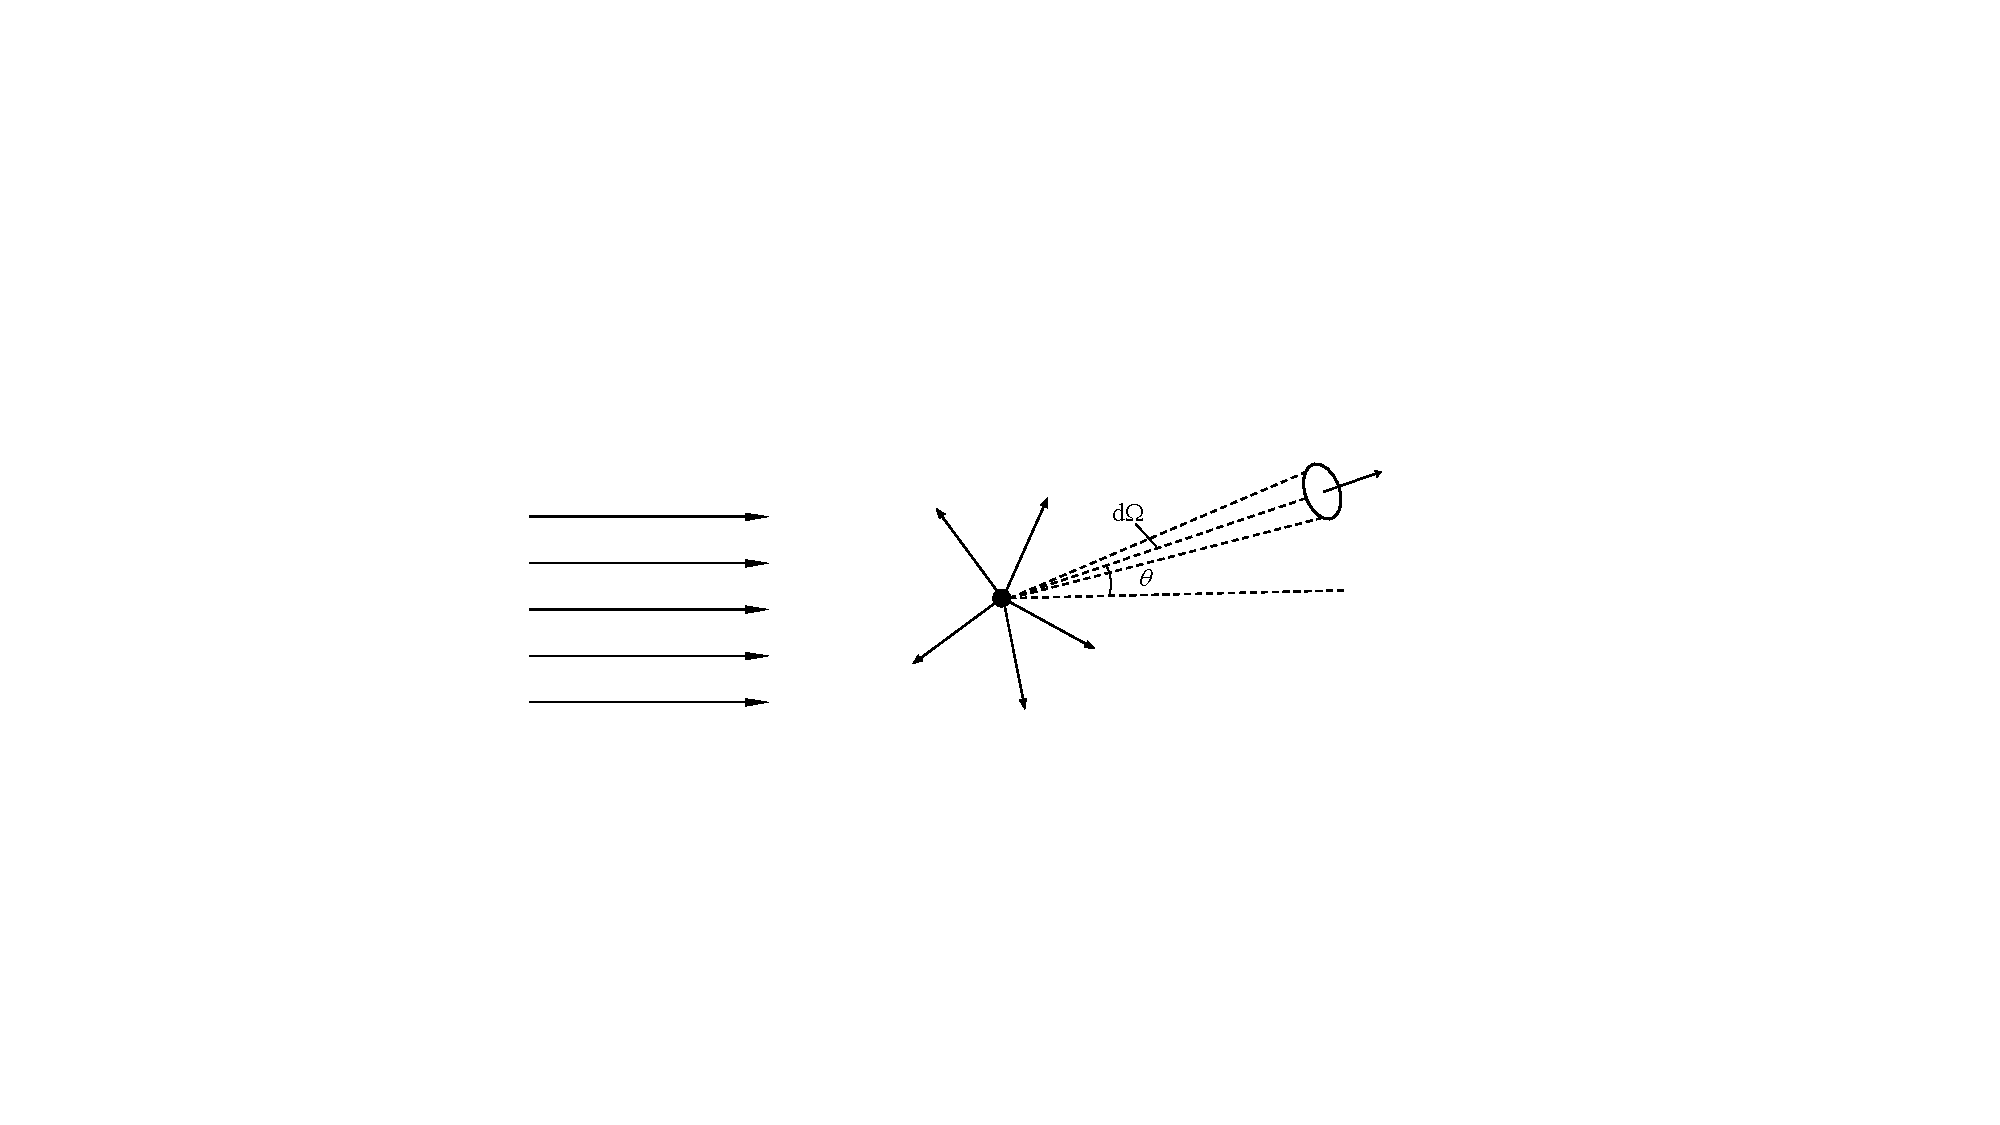
\includegraphics[width=6cm,clip]{QM file/figure/8-1}
	\caption{}\label{fig.8-1}
\end{figure}
粒子运动方向的偏转角称为散射角,即图中$\theta$.考虑一束速度为$v$的入射粒子,入射流量(入射方向单位横截面上,单位时间内通过的粒子数)为$N_{0}$,单位时间内散射的(改变了运动方向的)粒子数为$N$,其中散射到角范围$d\Omega$内的粒子数为$dN$.显然$N$与$dN$均和$N_{0}$成正比,令
\eqshort
\begin{empheq}{align}
	dN &= N_{0}\sigma(\theta,\varphi)d\Omega	\label{eq81.1}	\\
	N  &= \int dN=\sigma_{\text{总}}N_{0}		\label{eq81.2}
\end{empheq}
$\sigma(\theta.\varphi)$与$\sigma_{\text{总}}$的量纲均为面积,$\sigma_{\text{总}}$称为有效总散射截面,意义为,就散射的总效果而言,靶粒子(作用势$V$)相当于挡在入射粒子前进路上的一块横截面$\sigma_{\text{总}}$.$\sigma(\theta,\varphi)$称为有效微分散射截面,它和角元$d\Omega$所处的方向有关,其值取决于作用势$V$的性质.显然
\begin{empheq}{equation}\label{eq81.3}
	\sigma_{\text{总}}=\int\sigma(\theta,\varphi)d\Omega
\end{empheq}
在散射实验中,$N_{0}$和$dN/d\Omega$可以直接测量出来,再利用\eqref{eq81.1}式就得到$\sigma(\theta,\varphi)$的实验值,再由\eqref{eq81.3}式得到$\sigma$的实验值.散射理论的一项主要内容就是建立一套计算$\sigma(\theta,\varphi)$的理论方法,通过理论和实验的比较研究作用势$V$的性质.

{\heiti 2. 散射振幅}

作为散射过程的量子力学描述,入射粒子束可以近似地用平面波描述.以入射方向为$z$轴方向,入射粒子的动量表示成
\begin{empheq}{equation}\label{eq81.4}
	p=\mu v=\hbar k
\end{empheq}
则入射波为
\begin{empheq}{equation}\label{eq81.5}
	\varPsi_{i}=e^{ikz}
\end{empheq}\eqnormal
入射粒子数流量规定成
\begin{empheq}{align}\label{eq81.6}
	N_{0} &=j_{i}=-\frac{i\hbar}{2\mu}\bigg(\varPsi_{i}^{*}\frac{\partial}{\partial r}\varPsi_{i}-\varPsi_{i}\frac{\partial}{\partial r}\varPsi_{i}^{*}\bigg)	\nonumber\\
	&=\frac{\hbar k}{\mu}=v
\end{empheq}
($\varPsi_{i}^{*}\varPsi_{i}=1$,即规定单位体积内入射粒子数为1)
\noindent 散射过程的总波函数$\varPsi$可以表示成入射波$\varPsi_{i}$与散射波$\varPsi_{s}$之和,
\begin{empheq}{equation}\label{eq81.7}
	\varPsi=\varPsi_{i}+\varPsi_{s}=e^{ikz}+\varPsi_{s}
\end{empheq}
对于弹性散射,能量守恒,$\varPsi$满足定态薛定谔方程
\begin{empheq}{equation}\label{eq81.8}
	-\frac{\hbar^{2}}{2\mu}\nabla^{2}\varPsi+V(\boldsymbol{r})\varPsi=E\varPsi
\end{empheq}
其中$E=\frac{p^{2}}{2\mu}=\frac{\hbar^{2}k^{2}}{2\mu}$.通常,散射作用势$V$仅在小范围内起作用,$r\rightarrow\infty$处$V$迅速趋于0,这时\eqref{eq81.8}式变成自由粒子方程:
\begin{empheq}{equation}\label{eq81.9}
	\nabla^{2}\varPsi+k^{2}\varPsi\approx0\quad (r\rightarrow\infty)
\end{empheq}
入射波$\varPsi_{i}$是\eqref{eq81.9}式的一个严格解.$r\rightarrow\infty$处散射波$\varPsi_{s}$应该是\eqref{eq81.9}式的近似解,并取由散射中心$(r=0)$向外传播的球面波形式,即
\begin{empheq}{equation}\label{eq81.10}
	\varPsi_{s}\sim f(\theta,\varphi)\frac{e^{ikr}}{r}\quad (r\rightarrow\infty)
\end{empheq}
其中$f(\theta,\varphi)$称为散射振幅,它与方向$(\theta,\varphi)$有关.容易验证,当$r\rightarrow\infty$,如果略去$r^{-2}$以下小量,则不论$f(\theta,\varphi)$取什么函数形式,\eqref{eq81.10}式都能满足\eqref{eq81.9}式.这表明,在远离散射中心处$(r\rightarrow\infty)$,散射粒子又回到自由运动状态,\eqref{eq81.10}式正是自由粒子外向球面波波函数的一般近似表达式.(略去$r^{-2}$以下小量)一般需要解\eqref{eq81.8}式才能求得散射振幅$f(\theta,\varphi)$.

实验测量是在远离散射中心处进行的,相当于$r\rightarrow\infty$.如果略去$r^{-3}$以下小量,散射粒子数流量为
\begin{empheq}{align*}
	j_{s} &=-\frac{i\hbar}{2\mu}\bigg(\varPsi_{s}^{*}\frac{\partial}{\partial r}\varPsi_{s}-\varPsi_{s}\frac{\partial}{\partial r}\varPsi_{s}^{*}\bigg)	\\
	&=v|f(\theta,\varphi)|^{2}\bigg/ r^{2}
\end{empheq}
在角元$d\Omega$的横截面$r^{2}d\Omega$上单位时间内通过的散射粒子数为
\begin{empheq}{equation}\label{eq81.11}
	dN=j_{s}r^{2}d\Omega=v|f(\theta,\varphi)|^{2}d\Omega
\end{empheq}
与\eqref{eq81.1}式、\eqref{eq81.6}式比较,即得
\begin{empheq}{equation}\label{eq81.12}
	\sigma(\theta,\varphi)=|f(\theta,\varphi)|^{2}
\end{empheq}
散射理论的一项基本内容就是设法求出散射振幅$f(\theta,\varphi)$,从而算出微分散射截面$\sigma(\theta,\varphi)$.

{\heiti 3. 散射过程的经典力学描述}

在经典力学中,每个粒子均有一条运动轨道.以中心力场$V(r)$造成的散射为例,粒子的运动轨迹是一条平面曲线($\varphi$角不变),入射方向与出射方向的夹角就是散射角$\sigma$,如图\ref{fig.8-2}所示.散射角$\sigma$由碰撞参数(瞄准距离)$\rho$决定.经由横截面元$|\rho d\varphi d\rho|$的入射粒子,散射后进入$\theta$方向附近$d\Omega$角范围内,亦即
\begin{empheq}{equation}\label{eq81.13}
	dN=N_{0}|\rho d\rho d\varphi|=N_{0}\sigma(\theta)|d\Omega|
\end{empheq}

\begin{figure}[!h]
	\centering
	\small
	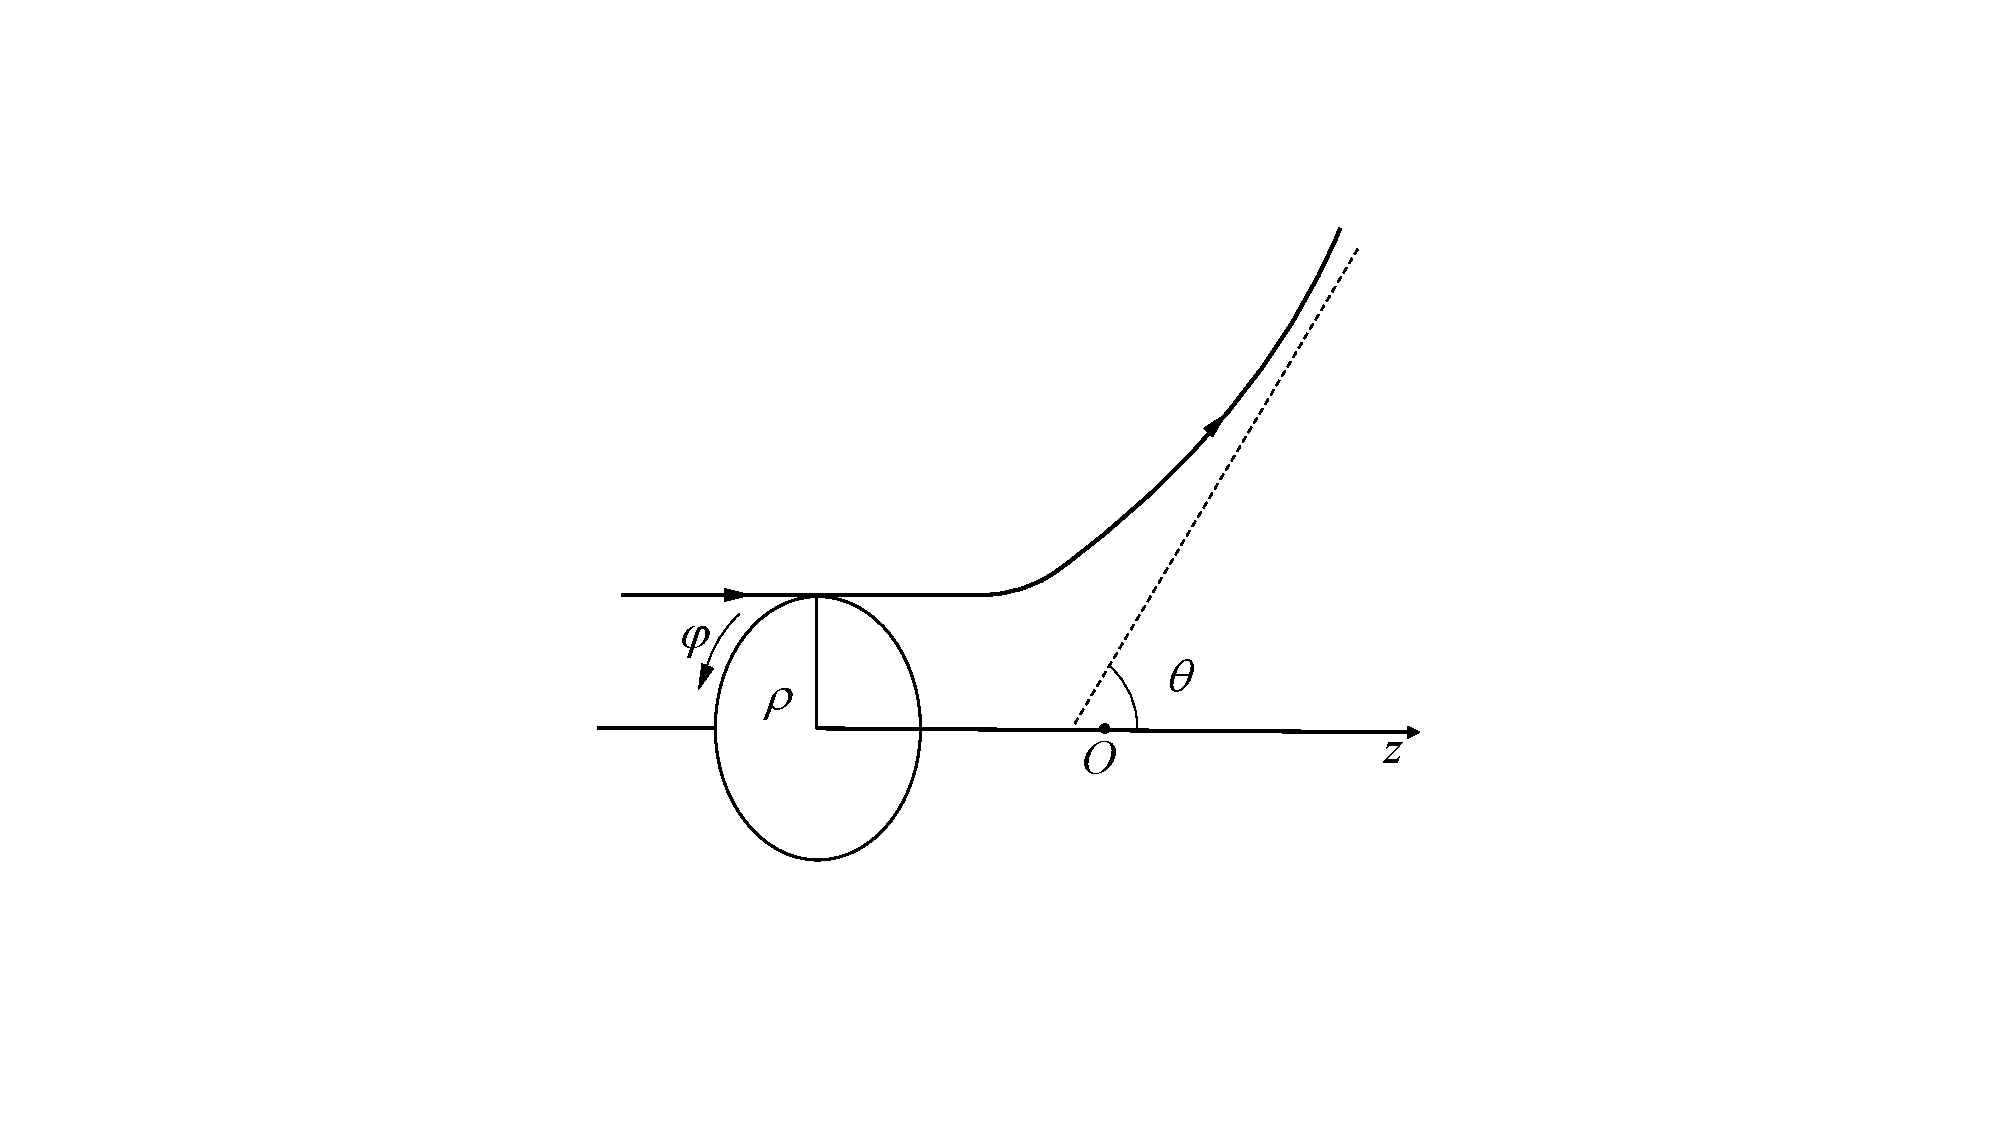
\includegraphics[width=4cm,clip]{QM file/figure/8-2}
	\caption{}\label{fig.8-2}
\end{figure}
其中$d\Omega=\sin\theta d\theta d\varphi$.由上式可得微分散射截面$\sigma(\theta)$的经典力学公式
\begin{empheq}{equation}\label{eq81.14}
	\sigma(\theta)=\left|\frac{\rho d\rho}{\sin\theta d\theta}\right|		%\bigg|\frac{\rho d\rho}{\sin\theta d\theta}\bigg|
\end{empheq}
经典散射理论的核心问题就是求碰撞参数$\rho$与散射角$\theta$的函数关系,从而得到$\sigma(\theta)$的公式.
\pskip

\example 速度为$v$的粒子束被半径为$a$的刚体球散射,求经典弹性散射截面.

\solution 总散射截面显然等于刚球的几何截面$\pi a^{2}$.下面求微分散射截面$\sigma(\theta)$.粒子与刚球碰撞发生弹性散射,入射角等于反射角,由图\ref{fig.8-3}容易看出下列关系:

\begin{figure}[!h]
	\centering
	\small
	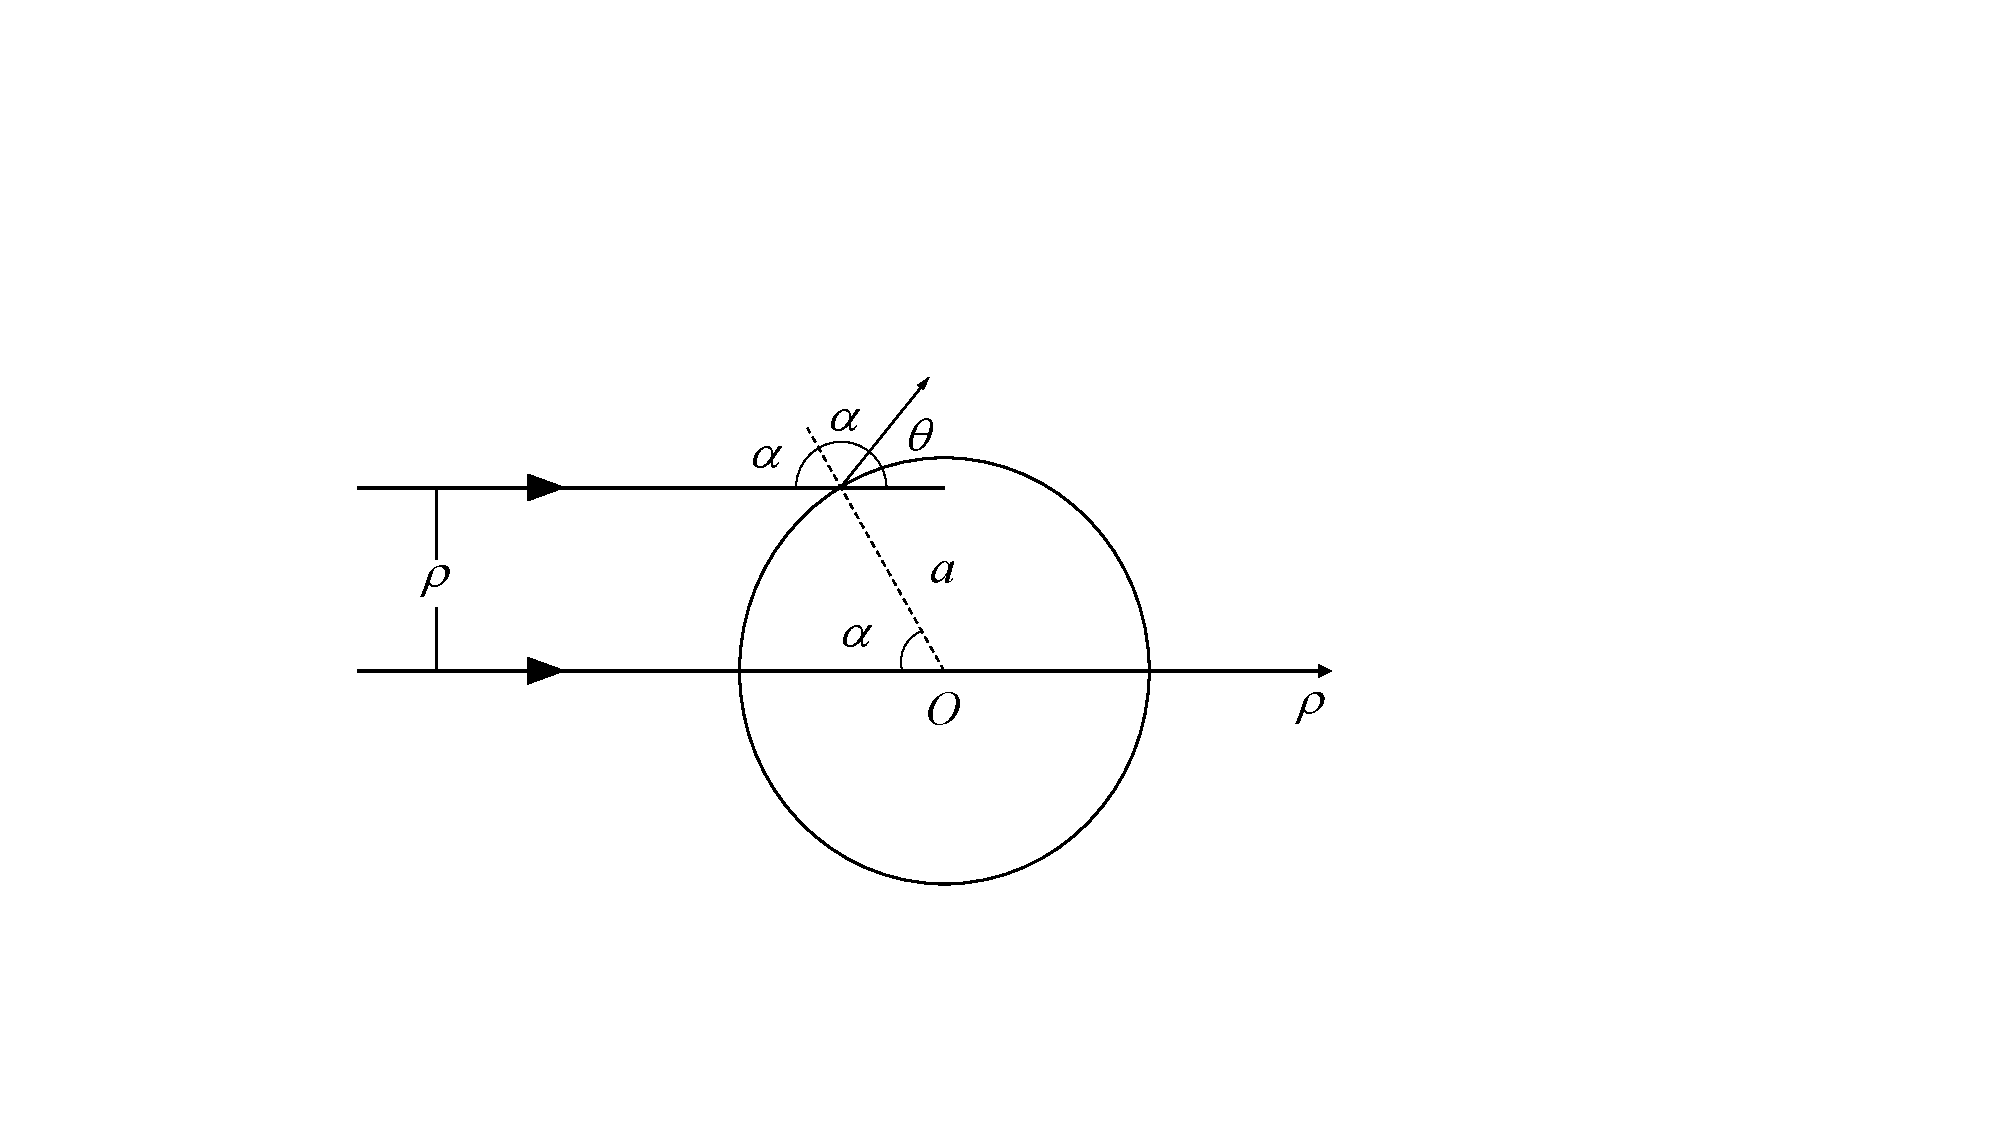
\includegraphics[width=5cm,clip]{QM file/figure/8-3}
	\caption{}\label{fig.8-3}
\end{figure}

\eqshort
\begin{empheq}{align*}
	&\theta+2\alpha=\pi	\\
	\rho= &a\sin\alpha=a \cos\frac{\theta}{2}
\end{empheq}\eqnormal
因此
\begin{empheq}{align*}
	\rho d\rho &=-\frac{a^{2}}{2}\cos\frac{\theta}{2}\sin\frac{\theta}{2}d\theta	\\
	&=-\frac{a^{2}}{4}\sin\theta d\theta
\end{empheq}
代入\eqref{eq81.14}式,即得
\eqshort
\begin{empheq}{equation}\label{eq81.15}
	\sigma(\theta)=a^{2}/4
\end{empheq}\eqnormal
$\sigma(\theta)$与$\theta$无关,这表示散射是各方向均匀的.显然
\begin{empheq}{align}\label{eq81.16}
	\sigma_{\text{总}} &=\int\sigma(\theta)d\Omega	\nonumber\\
		&= 4\pi\sigma(\theta)=\pi a^{2}
\end{empheq}



% 分波法
\section[分波法]{分波法} \label{sec:08.02} % 
% \makebox[5em][s]{} % 短题目拉间距

分波法是研究中心力场散射的普遍方法,其中心思想是将波函数展开成$(\boldsymbol{L}^{2},L_{z})$共同本征函数的线性叠加,然后逐项进行计算.

设散射作用势$V=V(r)$,与方向无关.这时粒子的轨道角动量$\boldsymbol{L}$是守恒量.取守恒量完全集为$(H,\boldsymbol{L}^{2},L_{z})$.入射波波函数的球坐标表示式为
\begin{empheq}{equation*}
	\varPsi_{i}=e^{ikz}=e^{ikr\cos\theta}
\end{empheq}
显然这是$L_{z}$的本征函数(本征值$m\hbar=0$),但不是$\boldsymbol{L}^{2}$的本征函数.如将$\varPsi_{k}$表示成$(\boldsymbol{L}^{2},L_{z})$共同本征函数$Y_{lm}$的线性叠加,可得[见\eqref{eq52.26}式]
\begin{empheq}{equation}\label{eq82.1}
	\varPsi_{i}=e^{ikr\cos\theta}=\sum_{l=0}^{\infty}(2l+1)e^{il\pi/2}j_{l}(kr)P_{l}(\cos\theta)
\end{empheq}
其中$P_{l}$是勒让德多项式,它与$Y_{l0}$只相差一个常系数,
\begin{empheq}{equation}\label{eq82.2}
	Y_{l0}=\sqrt{\frac{2l+1}{4\pi}}P_{l}(\cos\theta)
\end{empheq}
$j_{l}$是球贝塞耳函数,它是自由粒子球面波的径向波函数.我们将\eqref{eq82.1}式写成
\begin{empheq}{equation*}\label{eq82.1'}
	\varPsi=\frac{1}{kr}\sum_{l=0}^{\infty}u_{l}^{(0)}(r)Y_{l0}(\theta)
	\tag{$8.2.1^{\prime}$}
\end{empheq}
其中
\begin{empheq}{align}
	u_{l}^{(0)}&(r) =A_{l}^{(0)}krj_{l}(kr)			\label{eq82.3}\\
	A_{l}^{(0)}&=\sqrt{4\pi(2l+1)}e^{il\pi/2}		\label{eq82.4}
\end{empheq}
$u_{l}^{(0)}$满足自由粒子径向方程[见\eqref{eq52.4}式]
\begin{empheq}{equation}\label{eq82.5}
	\frac{d^{2}}{dr^{2}}u_{l}^{(0)}+\bigg[k^{2}-\frac{l(l+1)}{r^{2}}\bigg]u_{l}^{(0)}=0
\end{empheq}
根据$\S$\ref{sec:05.02}的讨论,$r\rightarrow\infty$处有下列渐近行为:
\begin{empheq}{align}
	j_{l}(kr)&\approx\frac{1}{kr}\sin\bigg(kr-\frac{l\pi}{2}\bigg)		\label{eq82.6}	\\
	u_{l}^{(0)}(r)&\approx A_{l}^{(0)}\sin\bigg(kr-\frac{l\pi}{2}\bigg)		\nonumber	\tag{$8.2.6^{\prime}$}	\label{eq82.6'}
\end{empheq}
在入射波也中,第$l$项分波($Y_{l0}$项)的相对比重显然与$|A_{l}^{(0)}|^{2}$成比例,亦即与$(2l+1)$成比例.在经典散射理论中,入射粒子束(参看图\ref{fig.8-2})的$L_{z}$仍为0,而$|\boldsymbol{L}|\propto\rho$,角动量值在$(L,L+\Delta L)$间的入射粒子数与$2\pi\rho\Delta\rho$成比例,亦即与$L\Delta L$成比例,如取$\Delta L=\hbar$,以及
\begin{empheq}{equation*}
	L\sim \sqrt{l(l+1)}\hbar\sim \bigg(l+\frac{1}{2}\bigg)\quad (l\gg 1)
\end{empheq}
则角动量取某个$L$值的入射粒子数与$L$成比例,并大致与$\bigg(l+\frac{1}{2}\bigg)$成比例,这个结论和量子力学结论一致.

经过散射后的总波函数$\varPsi$满足定态薛定谔方程
\begin{empheq}{equation}\label{eq82.7}
	-\frac{\hbar^{2}}{2\mu}\nabla^{2}\varPsi+V(r)\varPsi=\frac{\hbar^{2}k^{2}}{2\mu}\varPsi
\end{empheq}
由于是中心力场,$\boldsymbol{L}^{2},L_{z}$守恒,$l,m$是好量子数,其取值及概率分布不受$V(r)$的影响,如将$\varPsi$表示成$(H,\boldsymbol{L}^{2},L_{z})$共同本征函数的线性叠加,将是
\begin{empheq}{equation}\label{eq82.8}
	\varPsi(r,\theta)=\frac{1}{kr}\sum_{l=0}^{\infty}u_{l}(r)Y_{l0}(\theta)
\end{empheq}
$\varPsi$与$\varPsi_{i}$的差别在于$u_{l}^{(0)}$变成了$u_{l}$,后者满足径向方程
\begin{empheq}{equation}\label{eq82.9}
	\frac{d^{2}}{dr^{2}}u_{l}+\left[k^{2}-\frac{l(l+1)}{r^{2}}-\frac{2\mu}{\hbar^{2}}V(r)\right]u_{l}=0
\end{empheq}
给定$V(r)$后,由上式即可解出$u_{l}$.下面讨论$r\rightarrow\infty$处$u_{l}$的渐近行为.$r\rightarrow\infty$处$V(r)$一般均迅速趋于0,这时\eqref{eq82.9}式中$V(r)$及离心势($r^{-2}$项)均可略去,成为
\begin{empheq}{equation}\label{eq82.10}
	\frac{d^{2}}{dr^{2}}u_{l}+k^{2}u_{l}\approx 0
\end{empheq}
其渐近解为
\begin{empheq}{equation}\label{eq82.11}
	u_{l}(r)\approx A\sin\left(kr-\frac{l\pi}{2}+\delta_{l}\right)
\end{empheq}
$A_{l}$和$\delta_{l}$是待定常数.将\eqref{eq82.11}式和\eqref{eq82.6'}式比较,可知$u_{l}^{(0)}$与$u_{l}$的渐近性质存在两方面的差别:

(i) 振幅由$A_{l}^{(0)}$变成$A_{l}$;

(ii) $u_{l}$的渐近形式中增添了“相移”$\delta_{l}$.
当然,这都是散射造成的后果.

将\eqref{eq82.6'}式代入\eqref{eq82.1'}式,并利用公式
\begin{empheq}{equation*}
	\sin x=\frac{e^{ix}-e^{-ix}}{2i}
\end{empheq}
可得$r\rightarrow\infty$处$\varPsi_{i}$的渐近形式
\eqlong
\begin{empheq}{equation}\label{eq82.12}
	\varPsi_{i}\approx\frac{1}{2ikr}\sum_{l}A_{l}^{(0)}(e^{ikr}e^{-il\pi/2}-e^{-ikr}e^{il\pi/2})Y_{l0}(\theta)
\end{empheq}
而将\eqref{eq82.11}式代入\eqref{eq82.8}式可得$\varPsi$的渐近形式
\begin{empheq}{equation}\label{eq82.13}
	\varPsi_{i}\approx\frac{1}{2ikr}\sum_{l}A_{l}[e^{ikr}e^{i(\delta_{l}-l\pi/2)}-e^{-ikr}e^{i(l\pi/2-\delta_{l})}]Y_{l0}(\theta)
\end{empheq}\eqnormal
由于
\begin{empheq}{equation}\label{eq82.14}
	\varPsi-\varPsi_{i}=\varPsi_{s}\approx f(\theta)\frac{e^{ikr}}{r}
\end{empheq}
\eqref{eq82.12}式和\eqref{eq82.13}式中$e^{-ikr}$项应该相同,由此可知
\begin{empheq}{equation}\label{eq82.15}
	A_{l}=A_{l}^{(0)}e^{i\delta_{l}}
\end{empheq}
以及
\begin{empheq}{equation*}
	f(\theta)=\frac{1}{2ik}\sum_{l}(A_{l}e^{i\delta_{l}}-A_{l}^{(0)})e^{-il\pi/2}Y_{l0}(\theta)
\end{empheq}
将\eqref{eq82.4}式及\eqref{eq82.15}式代入上式,经过化简,即得散射振幅$f(\theta)$与各分波相移$\delta_{l}$的关系式
\begin{empheq}{align}\label{eq82.16}
	f(\theta) &=\frac{\sqrt{4\pi}}{k}\sum_{l=0}^{\infty}\sqrt{2l+1}\sin\delta_{l}e^{i\delta_{l}}Y_{l0}(\theta)		\nonumber\\
	&=\frac{1}{k}\sum_{l=0}^{\infty}(2l+1)\sin\delta_{l}e^{i\delta_{l}}P_{l}(\cos\theta)	\nonumber\\
	&=\sum_{l=0}^{\infty}f_{l}(\theta)
\end{empheq}
其中$f_{l}(\theta)$为第$l$个分波造成的散射振幅,即
\begin{empheq}{equation}\label{eq82.17}
	\frac{1}{kr}[u_{l}-u_{l}^{(0)}]Y_{l0}(\theta)\approx f_{l}(\theta)\frac{e^{ikr}}{r}
\end{empheq}
在散射过程中,各个分波各自独立地产生相移$\delta_{l}$,并对散射振幅作出独立的贡献.根据\eqref{eq81.12}式,微分散射截面为
\begin{empheq}{equation}\label{eq82.18}
	\sigma(\theta)=f^{*}(\theta)f(\theta)
\end{empheq}
散射振幅及微分散射截面均与$\varphi$角无关,散射结果呈轴对称分布(以$z$轴为对称轴),这是中心力散射的特点.

如用各分波散射振幅来表示,$\sigma(\theta)$可以写成
\begin{empheq}{equation*}\label{eq82.18'}
	\sigma(\theta)=\sum_{l}\sum_{l^{\prime}}f_{l}^{*}(\theta)f_{l}(\theta)
	\tag{$8.2.18^{\prime}$}
\end{empheq}
各个分波散射振幅并不是对$\sigma(\theta)$作出独立的贡献,而是相互间存在干涉效应.总散射截面的构成情况则有所不同,由\eqref{eq81.3}式,
\begin{empheq}{align}\label{eq82.19}
	\sigma_{\text{总}} &=\int\sigma(\theta)d\Omega	\nonumber\\
	&= \sum_{l}\sum_{l^{\prime}}\int f_{l}^{*}(\theta)f_{l^{\prime}}(\theta)d\Omega
\end{empheq}
由于$f_{l}$中含有$Y_{l0}(\theta)$,而球谐函数具有正交性
\begin{empheq}{equation*}
	\int Y_{l0}^{*}(\theta)Y_{l^{\prime}0}(\theta)d\Omega=\delta_{ll^{\prime}}
\end{empheq}
因此\eqref{eq82.19}式中仅$l=l^{\prime}$的项对积分有贡献.容易算出
\begin{empheq}{align}
	\sigma_{\text{总}}=\sum_{l}&\int f_{l}^{*}(\theta)f_{l}(\theta)d\Omega=\sum_{l}\sigma_{l}	\label{eq82.20}\\
	\sigma_{l}=&\int f_{l}^{*}(\theta)f_{l}(\theta)d\Omega	\nonumber\\
	=&\frac{4\pi}{k^{2}}(2l+1)\sin^{2}\delta_{l}		\label{eq82.21}
\end{empheq}
在$\sigma_{\text{总}}$的构成中,干涉效应消失,各个分波各自独立地对$\sigma_{\text{总}}$作出贡献,$\sigma_{l}$称为第$l$分波的散射截面.

当散射角$\theta\rightarrow0$,散射振幅$f$的值有特殊意义.当$\theta\rightarrow0$,\eqref{eq82.16}式中$P_{l}(1)=1$,因此
\begin{empheq}{equation}\label{eq82.22}
	f(0)=\frac{1}{k}\sum_{l}(2l+1)\sin\delta_{l}e^{i\delta_{l}}=\sum_{l}f_{l}(0)
\end{empheq}
容易看出
\begin{empheq}{align}
	\sigma_{l} &=\frac{4\pi}{k}\lm f_{l}(0)		\label{eq82.23}	\\
	\sigma_{\text{总}} &=\frac{4\pi}{k}\lm f(0)		\label{eq82.24}
\end{empheq}
($\lm$表示取虚部)这个结果称为光学定理.

用分波法处理中心力散射,关键是先要求出各级分波相移$\delta_{l}$,然后由\eqref{eq82.16}式和\eqref{eq82.18}式就可得出散射振幅$f(\theta)$和微分散射截面$\sigma(\theta)$.求$\delta_{l}$的基本方法是解径向方程\eqref{eq82.9}式,并辅以各种近似方法.下面介绍一种计算$\delta_{l}$的近似公式.

以$u_{l}^{(0)}$左乘\eqref{eq82.9}式,$u_{l}$左乘\eqref{eq82.5}式,相减即得
\begin{empheq}{equation*}
	\frac{d}{dr}\left[u_{l}^{(0)}\frac{du_{l}}{dr}-u_{l}\frac{du_{l}^{(0)}}{dr}\right]=\frac{2\mu}{\hbar^{2}}V(r)u_{l}u_{l}^{(0)}
\end{empheq}
对$r$积分,得到
\eqlong
\begin{empheq}{equation*}
	\frac{2\mu}{\hbar^{2}}\int_{0}^{\infty}V(r)u_{l}u_{l}U(0)dr=\left[u_{l}^{(0)}\frac{du_{l}}{dr}-u_{l}\frac{du_{l}^{(0)}}{dr}\right]\big|_{r=0}^{r\rightarrow\infty}
\end{empheq}\eqnormal
当$r=0$,上式右端为0;当$r\rightarrow\infty$,由\eqref{eq82.6'}及\eqref{eq82.11}式,上式右端为$(-kA_{l}A_{l}^{(0)}\sin\delta_{l})$,因此
\begin{empheq}{equation}\label{eq82.25}
	\sin\delta_{l}=-\frac{2\mu}{\hbar^{2}kA_{l}A_{l}U(0)}\int_{0}^{\infty}V(r)u_{l}u_{l}U(0)dr
\end{empheq}
至此是严格的.如某个分波散射较弱,$|\delta_{l}|\ll 1$,(条件见下面的叙述)则上式中可以用$u_{l}^{(0)}$代替$u_{l}$,$A_{l}^{(0)}$代替$A_{l}$,从而得到
\begin{empheq}{equation}\label{eq82.26}
	\sin\delta_{l}\approx\delta_{l}\approx-\frac{2\mu k}{\hbar^{2}}\int_{0}^{\infty}V(r)[j_{l}(kr)]^{2}r^{2}dr
\end{empheq}
由上式容易看出,如果$V>O$(排斥力),则$\delta_{l}<0$;如果$V<O$(吸引力),则$\delta_{l}>0$.在许多场合,散射作用势$V$仅在一定距离内($r\leqslant a$,$a$称为作用球半径.)才有显著值,这时\eqref{eq82.26}式的积分上限可以换成$a$.这种情况下,按照经典散射模型,能够产生显著散射的最大碰撞参数为$\rho_{max}\approx a$,最大角动量为$L_{max}\approx\hbar ka$.常称$ka\gg 1$的情况为高能散射,这时需要考虑的分波数目较多$(l_{max}\gg 1)$,用分波法处理较为麻烦,$ka\ll 1$的情况称为低能散射,这时经典$L_{max}\ll\hbar$,用分波法处理只需考
虑$l=0$这一分波(所谓s波),即可获得散射的主要信息.对于低能s波散射,
\begin{empheq}{align}
	f(\theta) &\approx f_{0}=\frac{1}{k}\sin\delta_{0}e^{i\delta_{0}}		\label{eq82.27}	\\
	\sigma(\theta) &\approx |f_{0}|^{2}=\frac{1}{k^{2}}\sin^{2}\delta_{0}		\label{eq82.28}
\end{empheq}
散射的角分布是各向同性的.
\pskip

\example 刚体球散射的分波法处理.

刚体球(半径$a$)的量子力学含义是
\begin{empheq}{equation*}
	{V(r)=}
	\begin{dcases}
		0,\qquad  r>a	\\
		\infty, \quad r\leqslant a
	\end{dcases}
\end{empheq}
在球内区域$(r\leqslant a)$波函数$\varPsi=0$.入射波仍由\eqref{eq82.1}式表示,散射后总波函数仍由\eqref{eq82.8}式表示在球外区域$(r>0)V=0$,因此径向方程\eqref{eq82.9}式形式上和\eqref{eq82.5}式相同,亦即和\eqref{eq52.4}式相同.\eqref{eq82.9}式有两个独立解,一个就是$kr_{l}(kr)$;另一个解在$\S$\ref{sec:05.02}中曾经提到,但随即以$r\rightarrow0$处边界条件为由予以舍弃,这个解通常记为$krn_{l}(kr)$,$n_{l}$称为球诺依曼函数,其定义为
\begin{empheq}{align}\label{eq82.29}
	n_{l}(\rho) &=(-1)^{(l+1)}\sqrt{\frac{\pi}{2\rho}}J_{-l-\frac{1}{2}}(\rho)	\nonumber\\
	&= (-1)^{l+1}\rho^{l}\left(\frac{1}{\rho}\frac{d}{d\rho}\right)^{l}\frac{\cos\rho}{\rho}
\end{empheq}
亦即在$j_{l}(\rho)$的定义[\eqref{eq52.16}式]中将$\sin\rho$换成$(-\cos\rho)$,就成为$n_{l}(\rho)$.$\rho\rightarrow\infty$处$n_{l}$的渐近形式为
\begin{empheq}{equation}\label{eq82.30}
	n_{l}(\rho)\approx-\frac{1}{\rho}\cos\left(\rho-\frac{l\pi}{2}\right)
\end{empheq}
对于本题,在球外区域,第$l$分波的径向波函数应该取
\begin{empheq}{equation}\label{eq82.31}
	R_{l}(r)=\frac{u_{l}(r)}{kr}=c_{l}j_{l}(kr)+b_{l}n_{l}(kr)
\end{empheq}
$R_{l}$还必须满足边界条件$R_{l}(r=a)=0$,由此易得
\eqshort
\begin{empheq}{equation}\label{eq82.32}
	b_{l}/c_{l}=-\frac{j_{l}(ka)}{n_{l}(ka)}
\end{empheq}\eqnormal
当$r\rightarrow\infty$,$u_{l}$的渐近形式为
\begin{empheq}{equation*}
	u_{l}(r) \approx c_{l}\sin\bigg(kr-\frac{l\pi}{2}\bigg)-b_{l}\cos\bigg(kr-\frac{l\pi}{2}\bigg)
\end{empheq}
而由\eqref{eq82.11}式,
\eqlong
\begin{empheq}{align*}
	u_{l}(r) &\approx A_{l}\sin\bigg(kr-\frac{l\pi}{2}+\delta_{l}\bigg)	\\
	&=A_{l}\cos\delta_{l}\sin\bigg(kr-\frac{l\pi}{2}\bigg)+A_{l}\sin\delta_{l}\cos\bigg(kr-\frac{l\pi}{2}\bigg)
\end{empheq}\eqnormal
比较即得
\begin{empheq}{align}
	c_{l}&= A_{l}\cos\delta_{l},\quad b_{l}=-A_{l}\sin\delta_{l}		\label{eq82.33}	\\
	&\frac{b_{l}}{c_{l}}=-\frac{\sin\delta_{l}}{\cos\delta_{l}}=-\tan\delta_{l} 	\nonumber	\tag{$8.2.33^{\prime}$}\label{eq82.33'}
\end{empheq}
比较\eqref{eq82.32}式及\eqref{eq82.33'}式,得出
\begin{empheq}{equation}\label{eq82.34}
	\tan\delta_{l}=\frac{j_{l}(ka)}{n_{l}(ka)}=(-1)^{l+1}\frac{J_{l+\frac{1}{2}}(ka)}{J_{-l-\frac{1}{2}}(ka)}
\end{empheq}
给定$ka$后,$j_{l}(ka)$及$n_{l(ka)}$的值可由贝塞耳函数表查出,代入上式就可算出$\delta_{l}$,再代入\eqref{eq82.16}式和\eqref{eq82.18}式就得到$f(\theta$和$\sigma(\theta)$.

以上是严格的.下面讨论低能散射和高能散射两种极端情况.对于低能散射,$ka\ll 1$,这时
\begin{empheq}{align}
	j_{l}(ka) &\approx \frac{(ka)^{l}}{(2l+1)!!}			\label{eq82.35}\\
	n_{l}(ka) &\approx -\frac{(2l-1)!!}{(ka)^{l+1}}			\nonumber\\
	\tan\delta_{l} &\approx-\frac{(ka)^{2l+1}}{(2l+1)!!(2l-1)!!}			\label{eq82.36}
\end{empheq}
注意$|\tan\delta_{l}|\ll 1$,所以
\begin{empheq}{equation*}
	\delta_{l}\approx\sin\delta_{l}\approx\tan\delta_{l}\propto(ka)^{2l+1}
\end{empheq}
例如
\eqlong
\begin{empheq}{equation*}
	\delta_{0}=-ka,\quad \delta_{l}\approx -\frac{(ka)^{3}}{3},\quad \delta_{2}\approx-\frac{(ka)^{5}}{45} -\frac{(ka)^{5}}{45}
\end{empheq}\eqnormal
($\delta_{0}$是严格的)随着$l$的增加, $\delta_{l}$减小得很快,所以可以略去一切$l\neq0$的分波散射[$\sigma_{l}\propto\delta_{l}^{2}\propto(ka)^{4l+2}$],只计算s波$(l=0)$散射,结果是
\begin{empheq}{align}\label{eq82.37}
	&\delta_{0}=-ka,\quad f(\theta)\approx f_{0} \approx -ae^{ika}	\nonumber\\
	&\sigma(\theta) \approx a^{2},\quad \sigma_{\text{总}} \approx \sigma_{0} 4\pi a^{2}
\end{empheq}
和经典散射类似,散射角分布是各向同性的.但总散射截面等于球的表面积,为经典散射截面的4倍.

高能散射,$ka\ll 1$.按照经典力学,能够造成散射的最大角动量为$L_{max}=\hbar ka$,即$l_{max}\approx ka$.量子力学结论虽不完全相同,但有显著散射效果的分波其$l$值的量级仍不超过$ka$.[证明较复杂,从略.当$l\gg ka$,\eqref{eq82.35}式即可成立,则$\delta_{l}$仍由\eqref{eq82.36}式表示,这时容易证明$|\delta_{l}|\ll 1$,相应的分波散射截面可以忽略不计.]而当$ka>l$,渐近表示式\eqref{eq82.6}及\eqref{eq82.30}式即可成立,则由\eqref{eq82.34}式可得
\begin{empheq}{equation*}
	\tan\delta_{l} \approx -\frac{\sin\bigg(ka-\frac{l\pi}{2}\bigg)}{\cos\bigg(ka-\frac{l\pi}{2}\bigg)}=-\tan\bigg(ka-\frac{l\pi}{2}\bigg)
\end{empheq}
所以
\eqshort
\begin{empheq}{equation}\label{eq82.38}
	\delta_{l}\approx -\bigg(ka-\frac{l\pi}{2}\bigg)
\end{empheq}
由于$\delta_{l+1}\approx \delta_{l}+\frac{\pi}{2}$,所以
\begin{empheq}{equation*}
	\sin^{2}\delta_{l}+\sin^{2}\delta_{l+1}\approx 1
\end{empheq}\eqnormal
计算$\sigma_{\text{总}}$时,不妨取每一项$\sin^{2}\delta_{l}$的有效值为$\frac{1}{2}$,从而得到
\begin{empheq}{align}\label{eq82.39}
	\sigma_{\text{总}}&\approx \frac{4\pi}{k^{2}}\sum_{l=0}^{ka}\bigg(l+\frac{1}{2}\bigg)	\nonumber\\
	&\approx \frac{4\pi}{k^{2}}\cdot\frac{1}{2}(ka+1)^{2}\approx 2\pi a^{2}
\end{empheq}
其中一半来自经典散射,一半来自衍射.至于$\sigma(\theta)$,由于主要贡献来自于$l\gg 1$的分波,角分布近似于各方向均匀分布.[原因是$P_{l}(\cos\theta)$在$\pm1$间振荡$l$次.]




% 低能散射
\starthis\section[低能散射]{低能散射$^{*}$} \label{sec:08.03} % 
% \makebox[5em][s]{} % 短题目拉间距
% \starthis 章节加星

继续上节的讨论,设散射作用势$V(r)$是短程的,在作用球(半径$a$)以外$V\approx0$.令$E=\frac{\hbar^{2}k^{2}}{2\mu}$,并考虑低能散射,$ka\ll 1$.这时第$l$级分波相移$\delta_{l}$大致与$(ka)^{2l+1}$成比例.[参看\eqref{eq82.26}式和\eqref{eq82.35}式,以及刚球散射.]可以只考虑s波$(l=0)$散射,而略去其他分波$(l\geqslant1)$的贡献.s波径向方程为
\begin{empheq}{equation}\label{eq83.1}
	\frac{d^{2}}{dr^{2}}u_{0}+\bigg[k^{2}-\frac{2\mu}{\hbar^{2}}V(r)\bigg]u_{0}=0
\end{empheq}
取低能极限$E\rightarrow0(k\rightarrow0)$,并研究$r>a$处(作用球外)$u_{0}$的表现形式.这时$V\approx0$,\eqref{eq83.1}式成为
\eqshort
\begin{empheq}{equation}\label{eq83.2}
	\frac{d^{2}}{dr^{2}}u_{0}=0
\end{empheq}
解为
\begin{empheq}{equation}\label{eq83.3}
	u_{0}(r)=c\bigg(1-\frac{r}{a_{0}}\bigg)
\end{empheq}\eqnormal
$c$及$a_{0}$为常数,$a_{0}$称为“散射长度”,其意义稍后再加以说明.

根据\eqref{eq82.11}式,在作用球外应该有渐近形式
\begin{empheq}{align*}
	u_{0}(r) &\approx A_{0}\sin(kr+\delta_{0})	\\
	&=A_{0}\sin\delta_{0}(\cos kr+\cot\delta_{0}\cdot\sin kr)
\end{empheq}
在低能极限下,$k\rightarrow=,\cos kr\rightarrow1,\sin kr\rightarrow kr$,上式成为
\begin{empheq}{equation*}
	u_{0}(r) \approx A_{0}\sin\delta_{0}(1+kr\cot\delta_{0})
\end{empheq}
与\eqref{eq83.3}式比较,可知
\begin{empheq}{equation}\label{eq83.4}
	\boxed{k\cot\delta_{0}=-\frac{1}{a_{0}}\quad(k\rightarrow0)}
\end{empheq}
散射振幅的低能极限为
\begin{empheq}{align}\label{eq83.5}
	f(\theta) &\approx f_{0}=\frac{1}{k}\sin\delta_{0}e^{i\delta_{0}}	\nonumber\\
	&=\frac{1}{k\cot\delta_{0}-ik}=-\frac{a_{0}}{1+ika_{0}}
\end{empheq}
如散射长度$a_{0}$取有限值,则当$k\rightarrow0,k|a_{0}|\ll1$,\eqref{eq83.5}式即
\begin{empheq}{equation}\label{eq83.6}
	f(\theta) \approx-a_{0}\quad (k\rightarrow0)
\end{empheq}
这时\eqref{eq83.4}式给出
\begin{empheq}{equation}\label{eq83.7}
	-ka_{0}=\tan\delta_{0}\approx\sin\delta_{0}\approx\delta_{0}
\end{empheq}
散射截面为
\begin{empheq}{align}\label{eq83.8}
	\sigma(\theta)&=|f(\theta)|^{2}=a_{0}^{2}	\nonumber\\
	\sigma_{\text{总}}&=4\pi a_{0}^{2}
\end{empheq}
这种情况下势场$V(r)$的散射效果相当于半径为$a_{0}$的刚球.注意$\delta_{0}$与$k$成正比,$f(\theta),\sigma(\theta)$均与$k$无关,即与能量$E$无关.

如$a_{0}\rightarrow\pm\infty$,则\eqref{eq83.4}式给出
\begin{empheq}{equation}\label{eq83.9}
	k\cot\delta_{0}=0,\quad \delta_{0}=\frac{\pi}{2},\quad\text{或}\quad -\frac{\pi}{2}
\end{empheq}
而\eqref{eq83.5}式给出
\eqshort
\begin{empheq}{equation}\label{eq83.10}
	f(\theta)=\frac{i}{k}
\end{empheq}\eqnormal
因此
\begin{empheq}{equation}\label{eq83.11}
	\sigma_{\text{总}}=4\pi\sigma(\theta)=\frac{4\pi}{k^{2}}=\frac{2\pi\hbar^{2}}{\mu E}
\end{empheq}
散射截面与$E$成反比.当$E\rightarrow0,\sigma_{\text{总}}\rightarrow\infty$,称为“共振散射”.

\begin{figure}[!h]
	\centering
	\small
	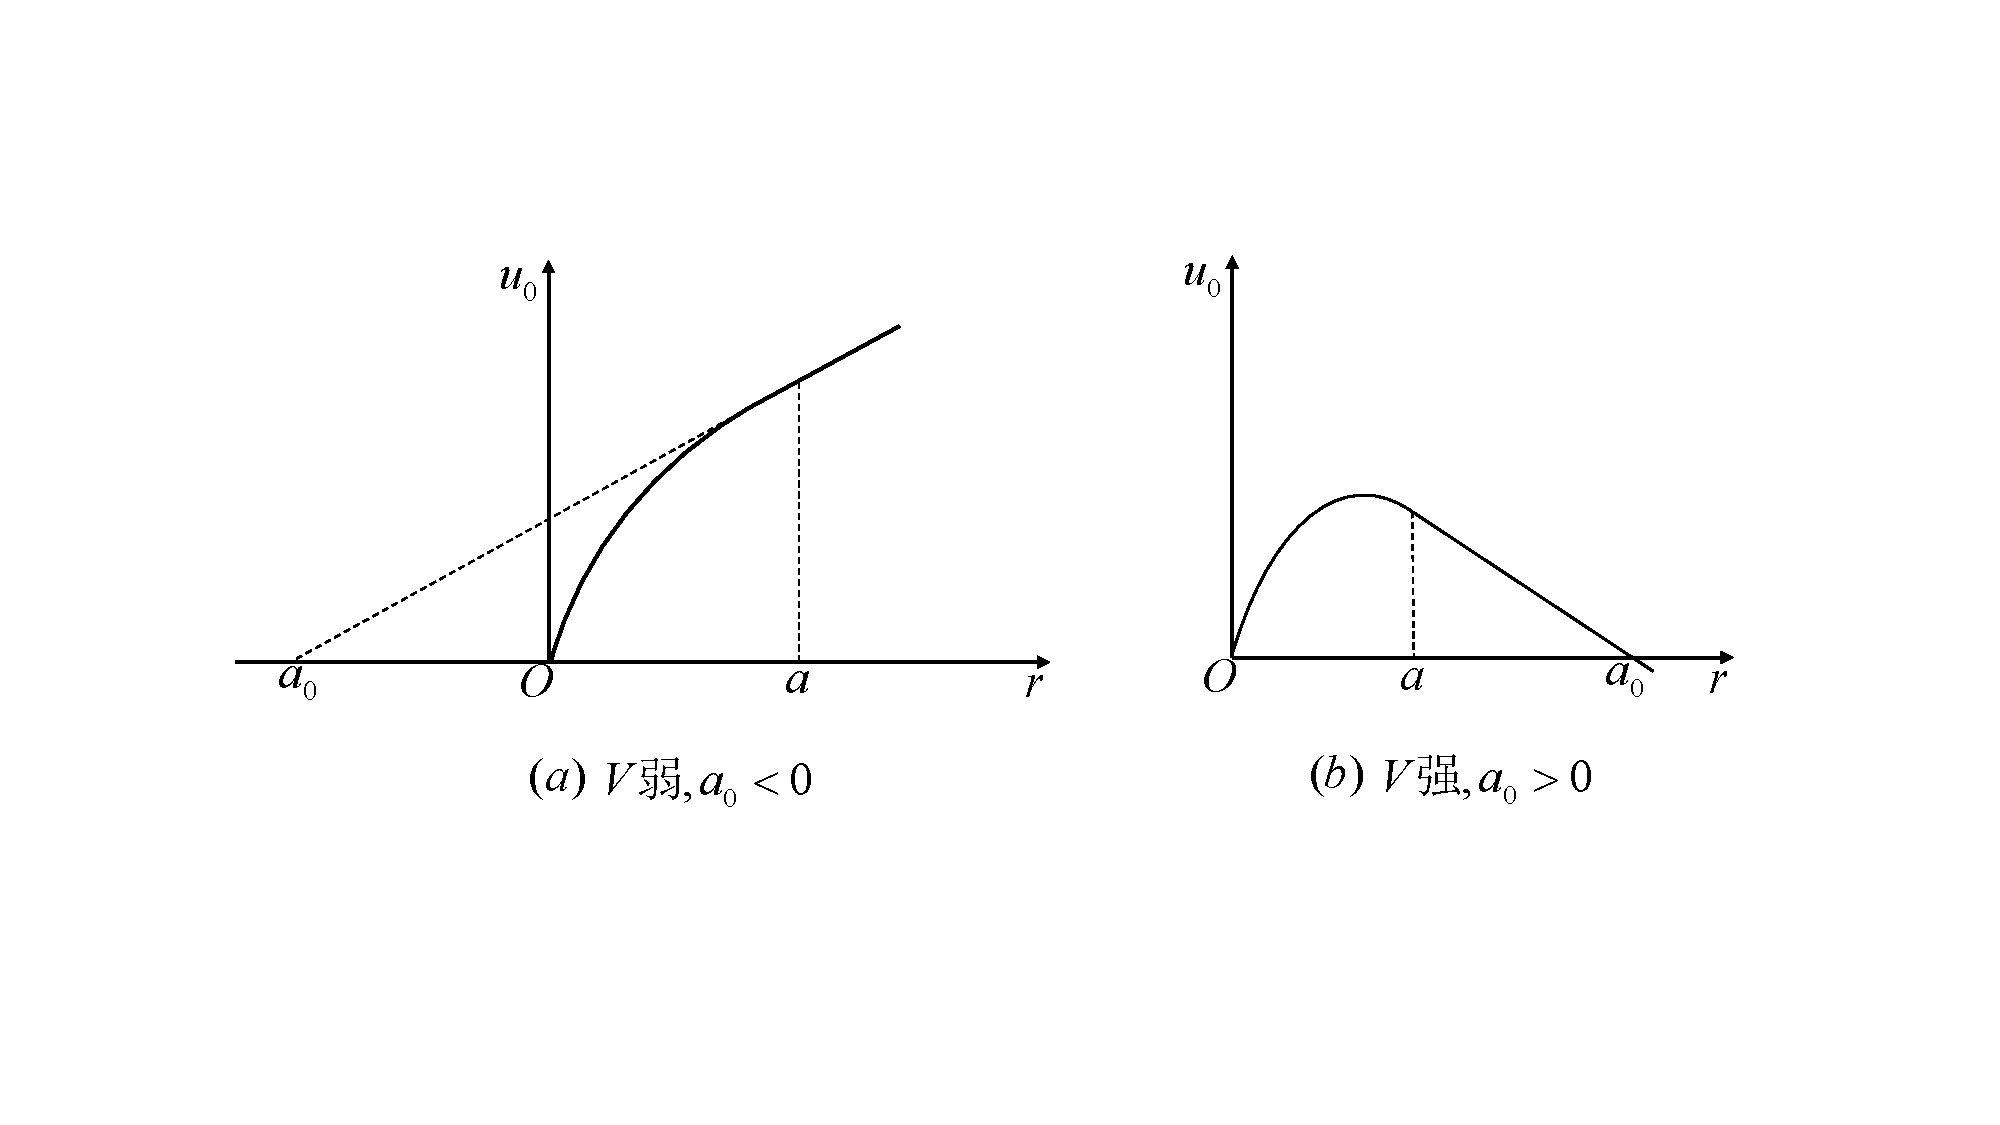
\includegraphics[width=7cm,clip]{QM file/figure/8-4}
	\caption{}\label{fig.8-4}
\end{figure}

下面以势阱$(V<0)$散射为例,说明散射长度的意义.当$E\rightarrow0$,由\eqref{eq83.1}式可知$\frac{u_{0}^{\prime\prime}}{u_{0}}$,$u_{0}$随$r$的变化如图\ref{fig.8-4}所示.如果作用势$V(r)$较弱,以致当$r$达到$a$(作用球半径)时$u_{0}$尚在上升阶段,$u_{0}^{\prime}$为正,则散射长度$a_{0}<0$.这种势阱不能造成束缚态.如果作用势$V(r)$较强,当$r$达到$a$时$u_{0}$已经处于下降阶段,$u_{0}^{\prime}$为负,则散射长度$a_{0}>0$.这种势阱可以造成束缚态能级$(E_{n}<0)$.而$a_{0}=\pm\infty$相当于$r=a$处$u_{0}^{\prime}=0$,这刚好是阱口出现束缚态能级$(E=0_{-})$的条件,这种情况下粒子的入射能量$(E\geqslant0)$接近于阱口附近的束缚态能级,在入射波与阱口束缚态之间容易产生共振跃迁,所以散射截面特别大.
\pskip

\example 讨论球形势阱

\begin{equation}\label{eq83.12}
	V(r)=
	\begin{cases}
		-V_{0},	& r<a	\\
		0,	& r>a
	\end{cases}
\end{equation}
造成的低能$(ka\ll1)$s波$(l=0)$散射.

\solution 令
\begin{empheq}{equation}\label{eq83.13}
	k=\frac{\sqrt{2\mu E}}{\hbar},\quad k_{0}=\frac{\sqrt{2\mu V_{0}}}{\hbar}
\end{empheq}
在阱内$(r<a)$,s波径向方程为
\eqshort
\begin{empheq}{equation}\label{eq83.14}
	u_{0}^{\prime\prime}+(k^{2}+k_{0}^{2})u_{0}=0
\end{empheq}\eqnormal
边界条件为$u_{0}(r=0)=0$.当$E\rightarrow0(k\rightarrow0)$,满足边界条件的解是
\begin{empheq}{equation}\label{eq83.15}
	u_{0}(r)=A\sin k_{0}r\quad (E\rightarrow0,r<a)
\end{empheq}
在阱外$(r>a)$,径向方程为
\eqshort
\begin{empheq}{equation*}
	u_{0}^{\prime\prime}+k^{2}u_{0}=0
\end{empheq}\eqnormal
当$E\rightarrow0$,解为
\begin{empheq}{equation}\label{eq83.16}
	u_{0}(r)=c\bigg(1-\frac{r}{a_{0}}\bigg)\quad (E\rightarrow0,r>a)
\end{empheq}
在$r=a$处,$\frac{u_{0}}{u_{0}^{\prime}}$应该连续,据此求出
\begin{empheq}{align}\label{eq83.17}
	\frac{1}{k}&\tan k_{0}a=a-a_{0}	\nonumber\\
	a_{0}=&-\frac{a(\tan k_{0}a-k_{0}a)}{k_{0}a}
\end{empheq}
$a_{0}$即散射长度.如$a_{0}$有限,由\eqref{eq83.8}式就得到散射截面(与$E$无关).

讨论:(i) 如势阱的性质($V_{0}$及$a$值)刚好使$\tan k_{0}a=k_{0}a$,这时$a_{0}=0$,低能极限下$(E\rightarrow0)\sigma_{\text{总}}\rightarrow0$,势阱是“透明”的.


(ii) 如势阱深而宽,$k_{0}a\gg 1$,同时$\tan k_{0}a$并不太大(非共振散射),这时$a_{0}=a,\sigma_{\text{总}}\approx4\pi a^{2}$,势阱的低能散射效果类似于刚球.


(iii) 如果$k_{0}a=\bigg(n+\frac{1}{2}\bigg)\pi(n=0,1,2,\cdots)$则当$E\rightarrow0$时出现共振散射$(a_{0}=\pm\infty)$.这时阱内区域粒子的德布罗意波长$\lambda_{0}\bigg(\approx\frac{2\pi}{k_{0}}\bigg)$与势阱半径$a$有关系
\eqshort
\begin{empheq}{equation}\label{eq83.18}
	2a=\bigg(n+\frac{1}{2}\bigg)\lambda_{0}
\end{empheq}\eqnormal
这也就是阱口出现束缚能级$(E=0_{-})$的条件.

(iv) 如果势阱浅而窄,$k_{0}a\ll 1$,则可取
\begin{empheq}{equation*}
	\tan k_{0}a\approx k_{0}a+\frac{1}{3}(k_{0}a)^{3}
\end{empheq}
由\eqref{eq83.17}式求得散射长度为
\begin{empheq}{equation}\label{eq83.19}
	a_{0}\approx -\frac{a}{3}(k_{0}a)^{2}=-\frac{2\mu V_{0}a^{3}}{3\hbar^{2}}
\end{empheq}
再由\eqref{eq83.7}式、\eqref{eq83.8}式得出
\begin{empheq}{align}
	\delta_{0}&=-k_{0}a=\bigg(\frac{2\mu V_{0}a^{2}}{3\hbar^{2}}\bigg)ak		\label{eq83.20}\\
	\sigma_{\text{总}}&=4\pi a_{0}^{2}=\frac{16\pi}{9}\bigg(\frac{\mu V_{0}a^{3}}{\hbar^{2}}\bigg)^{2}		\label{eq83.21}
\end{empheq}
如直接利用$\delta_{l}$的近似公式[\eqref{eq82.26}式],也可得到同样的结果.









% 玻恩近似
\section[玻恩近似]{玻恩近似} \label{sec:08.04} % 
% \makebox[5em][s]{} % 短题目拉间距

在弹性散射问题中,波函数表示成入射波和散射波的叠加,即
\begin{empheq}{equation}\label{eq84.1}
	\varPsi=e^{ikz}+\varPsi_{s}
\end{empheq}
$\varPsi$满足定态薛定谔方程,它可以写成
\begin{empheq}{equation}\label{eq84.2}
	(\nabla^{2}+k^{2})\varPsi=\frac{2\mu}{\hbar^{2}}V(\boldsymbol{r})\varPsi
\end{empheq}
其中$k=\frac{\sqrt{2\mu E}}{\hbar}$.\eqref{eq84.1}式中$e^{ikz}$为入射波,$\varPsi_{s}$为散射波,在$r\rightarrow\infty$处$\varPsi_{s}$取球面出射波的形式,即
\begin{empheq}{equation}\label{eq84.3}
	\varPsi_{s}\approx f(\theta,\varphi)\frac{e^{ikr}}{r}\quad (r\rightarrow\infty)
\end{empheq}
上式可以认为是$r\rightarrow\infty$处$\varPsi_{s}$满足的边界条件.

如作用势$V(r)$较弱,以致在作用球内就有$|\varPsi_{s}|<|e^{ikz}|$,我们可以视$V$为微扰,而对\eqref{eq84.2}式采用逐级近似解法.

{\heiti 1. 近似展开}

将总波函数$\varPsi$分解成零级近似,一级修正,二级修正,等等,令
\begin{empheq}{equation}\label{eq84.4}
	\varPsi=\varPsi^{(0)}+\varPsi^{(1)}+\varPsi^{(2)}+\cdots
\end{empheq}
零级近似取为入射波,即
\eqshort
\begin{empheq}{equation}\label{eq84.5}
	\varPsi^{(0)}=e^{ikz}
\end{empheq}\eqnormal
而散射波就是\eqref{eq84.4}式中其余各项之和,即
\begin{empheq}{equation}\label{eq84.6}
	\varPsi_{s}=\varPsi^{(1)}+\varPsi^{(2)}+\cdots
\end{empheq}
在$r\rightarrow\infty$处,各级修正项均应该取球面出射波的形式,即
\begin{empheq}{equation}\label{eq84.7}
	\begin{aligned}
		\varPsi^{(1)} &\approx f^{(1)}(\theta,\varphi)\frac{e^{ikr}}{r}	\\
		\varPsi^{(2)} &\approx f^{(2)}(\theta,\varphi)\frac{e^{ikr}}{r}
	\end{aligned}\qquad (r\rightarrow\infty)
\end{empheq}
等等与\eqref{eq84.3}式、\eqref{eq84.6}式比较,显然有
\begin{empheq}{equation}\label{eq84.8}
	f(\theta,\varphi)=f^{(1)}+f^{(2)}+\cdots
\end{empheq}
$f^{(1)}$和$f^{(2)}$就是散射振幅的一级近似和二级修正.

入射波$\varPsi^{(0)}$满足方程
\eqshort
\begin{empheq}{equation}\label{eq84.9}
	(\nabla^{2}+k^{2})\varPsi^{(0)}=0
\end{empheq}\eqnormal
因此\eqref{eq84.2}式化成
\eqindent{1}
\begin{empheq}{equation}\label{eq84.10}
	(\nabla^{2}+k^{2})(\varPsi^{(1)}+\varPsi^{(2)}+\cdots)=\frac{2\mu}{\hbar^{2}}V(\boldsymbol{r})(\varPsi^{(0)}+\varPsi^{(1)}+\varPsi^{(2)}+\cdots)
\end{empheq}\eqnormal
对上式用逐级近似解法,可令
\begin{empheq}{align}
	(\nabla^{2}+k^{2})\varPsi^{(1)}&=\frac{2\mu}{\hbar^{2}}V\varPsi^{(0)}		\label{eq84.11}	\\
	(\nabla^{2}+k^{2})\varPsi^{(2)}&=\frac{2\mu}{\hbar^{2}}V\varPsi^{(1)}		\label{eq84.12}
\end{empheq}
等等,先由\eqref{eq84.11}式解出$\varPsi^{(1)}$,再代入\eqref{eq84.12}式解出$\varPsi^{(2)}\cdots\cdots$依次逐级求解.

{\heiti 2. 格林函数}

\eqref{eq84.11}式的形式解可以写成
\begin{empheq}{equation*}\label{eq84.11'}
	\varPsi^{(1)}(\boldsymbol{r})=\frac{2\mu}(\nabla^{2}+k^{2})^{-1}V(\boldsymbol{r})\varPsi^{(0)}(\boldsymbol{r})
	\tag{$8.4.11^{\prime}$}
\end{empheq}
这里$(\nabla^{2}+k^{2})^{-1}$按照算符来理解,但其性质有待明确.引入$\delta$函数$\delta(\boldsymbol{r}-\boldsymbol{r}^{\prime})$,规定其性质为(这里和以下,凡是三重积分均指“全空间”积分)
\begin{empheq}{equation}\label{eq84.13}
	\int\rho(\boldsymbol{r}^{\prime})\delta(\boldsymbol{r}-\boldsymbol{r}^{\prime})d^{3}\boldsymbol{r}^{\prime}=\rho(\boldsymbol{r})
\end{empheq}
$\rho(\boldsymbol{r})$为任何具有良好积分收敛性的连续函数.再引入格林函数
\begin{empheq}{equation}\label{eq84.14}
	G(\boldsymbol{r},\boldsymbol{r}^{\prime})=(\nabla^{2}+k^{2})^{-1}\delta(\boldsymbol{r}-\boldsymbol{r}^{\prime})
\end{empheq}
则有
\begin{empheq}{align}\label{eq84.15}
	\int& G(\boldsymbol{r},\boldsymbol{r}^{\prime})\rho(\boldsymbol{r}^{\prime})d^{3}\boldsymbol{r}^{\prime}	\nonumber\\
	&=(\nabla^{2}+k^{2})^{-1}\int\delta(\boldsymbol{r}-\boldsymbol{r}^{\prime})\rho(\boldsymbol{r}^{\prime})d^{3}\boldsymbol{r}^{\prime}	\nonumber\\
	&=(\nabla^{2}+k^{2})^{-1}\rho(\boldsymbol{r})
\end{empheq}
因此\eqref{eq84.11'}式形式上可以写成
\begin{empheq}{equation}\label{eq84.16}
	\boxed{\varPsi^{(1)}(\boldsymbol{r})=\frac{2\mu}{\hbar^{2}}\int G(\boldsymbol{r},\boldsymbol{r}^{\prime})V(\boldsymbol{r}^{\prime})\varPsi^{(0)}(\boldsymbol{r}^{\prime})d^{3}\boldsymbol{r}^{\prime}}
\end{empheq}
注意,\eqref{eq84.14}式仅是格林函数的形式定义,其实质就是
\begin{empheq}{equation}\label{eq84.14'}
	(\nabla^{2}+k^{2})G(\boldsymbol{r},\boldsymbol{r}^{\prime})=\delta(\boldsymbol{r}-\boldsymbol{r}^{\prime})
	\tag{$8.4.14^{\prime}$}
\end{empheq}
将齐次方程$(\nabla^{2}+k^{2})u=0$的任何一个解加入$G(\boldsymbol{r},\boldsymbol{r}^{\prime})$中,显然仍满足\eqref{eq84.14'}式.在具体问题中,选取$G(\boldsymbol{r},\boldsymbol{r}^{\prime})$的函数形式时应该根据问题的性质,并满足相应的边界条件.对于散射问题,可取
\begin{empheq}{equation}\label{eq84.17}
	\delta(\boldsymbol{r}-\boldsymbol{r}^{\prime})=\frac{1}{(2\pi)^{3}}\int\exp[i\boldsymbol{k}^{\prime}\cdot(\boldsymbol{r}-\boldsymbol{r}^{\prime})]d^{3}\boldsymbol{k}^{\prime}
\end{empheq}
由于
\begin{empheq}{equation*}
	(\nabla^{2}+k^{2})e^{i\boldsymbol{k}^{\prime}\cdot\boldsymbol{r}}=(k^{2}-k^{\prime2})e^{i\boldsymbol{k}^{\prime}\cdot\boldsymbol{r}}
\end{empheq}
格林函数可以取为
\eqlong
\begin{empheq}{equation}\label{eq84.18}
	G(\boldsymbol{r},\boldsymbol{r}^{\prime})=\frac{1}{(2\pi)^{3}}\int\frac{d^{3}\boldsymbol{k}^{\prime}}{k^{2}-k^{\prime2}}\exp[i\boldsymbol{k}^{\prime}\cdot(\boldsymbol{r}-\boldsymbol{r}^{\prime})]
\end{empheq}\eqnormal
上式中积分在$\boldsymbol{k}^{\prime}$空间进行,$k,\boldsymbol{r},\boldsymbol{r}^{\prime}$作为参量对待.如在$\boldsymbol{k}^{\prime}$空间取球坐标$(k^{\prime},\theta,\varphi)$,并以$(\boldsymbol{r}-\boldsymbol{r}^{\prime})$作为极轴,则
\begin{empheq}{equation*}
	d^{3}\boldsymbol{k}^{\prime}=k^{\prime2}dk^{\prime}\sin\theta d\theta d\varphi
\end{empheq}
\eqref{eq84.18}式中角部积分容易算出,为
\begin{empheq}{align}\label{eq84.19}
	\int&\exp[i\boldsymbol{k}^{\prime}\cdot(\boldsymbol{r}-\boldsymbol{r}^{\prime})]\sin\theta d\theta d\varphi		\nonumber\\
	&=\int_{0}^{2\pi}d\varphi\int_{0}^{\pi}\exp[ik^{\prime}|\boldsymbol{r}-\boldsymbol{r}^{\prime}|\cos\theta]\sin\theta d\theta	\nonumber\\
	&=4\pi\frac{\sin(k^{\prime}|\boldsymbol{r}-\boldsymbol{r}^{\prime}|)}{k^{\prime}|\boldsymbol{r}-\boldsymbol{r}^{\prime}|}
\end{empheq}
代入\eqref{eq84.18}式,得到
\eqindent{1}
\begin{empheq}{align}\label{eq84.20}
	G&(\boldsymbol{r},\boldsymbol{r}^{\prime})=\frac{1}{2\pi^{2}}\cdot\frac{1}{|\boldsymbol{r}-\boldsymbol{r}^{\prime}|}\int_{0}^{\infty}\frac{k^{\prime}dk^{\prime}}{k^{2}-k^{\prime}}\sin(k^{\prime}|\boldsymbol{r}-\boldsymbol{r}^{\prime}|)	\nonumber\\
	&=\frac{i}{8\pi^{2}|\boldsymbol{r}-\boldsymbol{r}^{\prime}|}\int_{-\infty}^{\infty}\bigg(\frac{1}{k^{\prime}+k}+\frac{1}{k^{\prime}-k}\bigg)\exp(ik^{\prime}|\boldsymbol{r}-\boldsymbol{r}^{\prime}|)dk^{\prime}
\end{empheq}\eqnormal

\begin{figure}[!h]
	\centering
	\small
	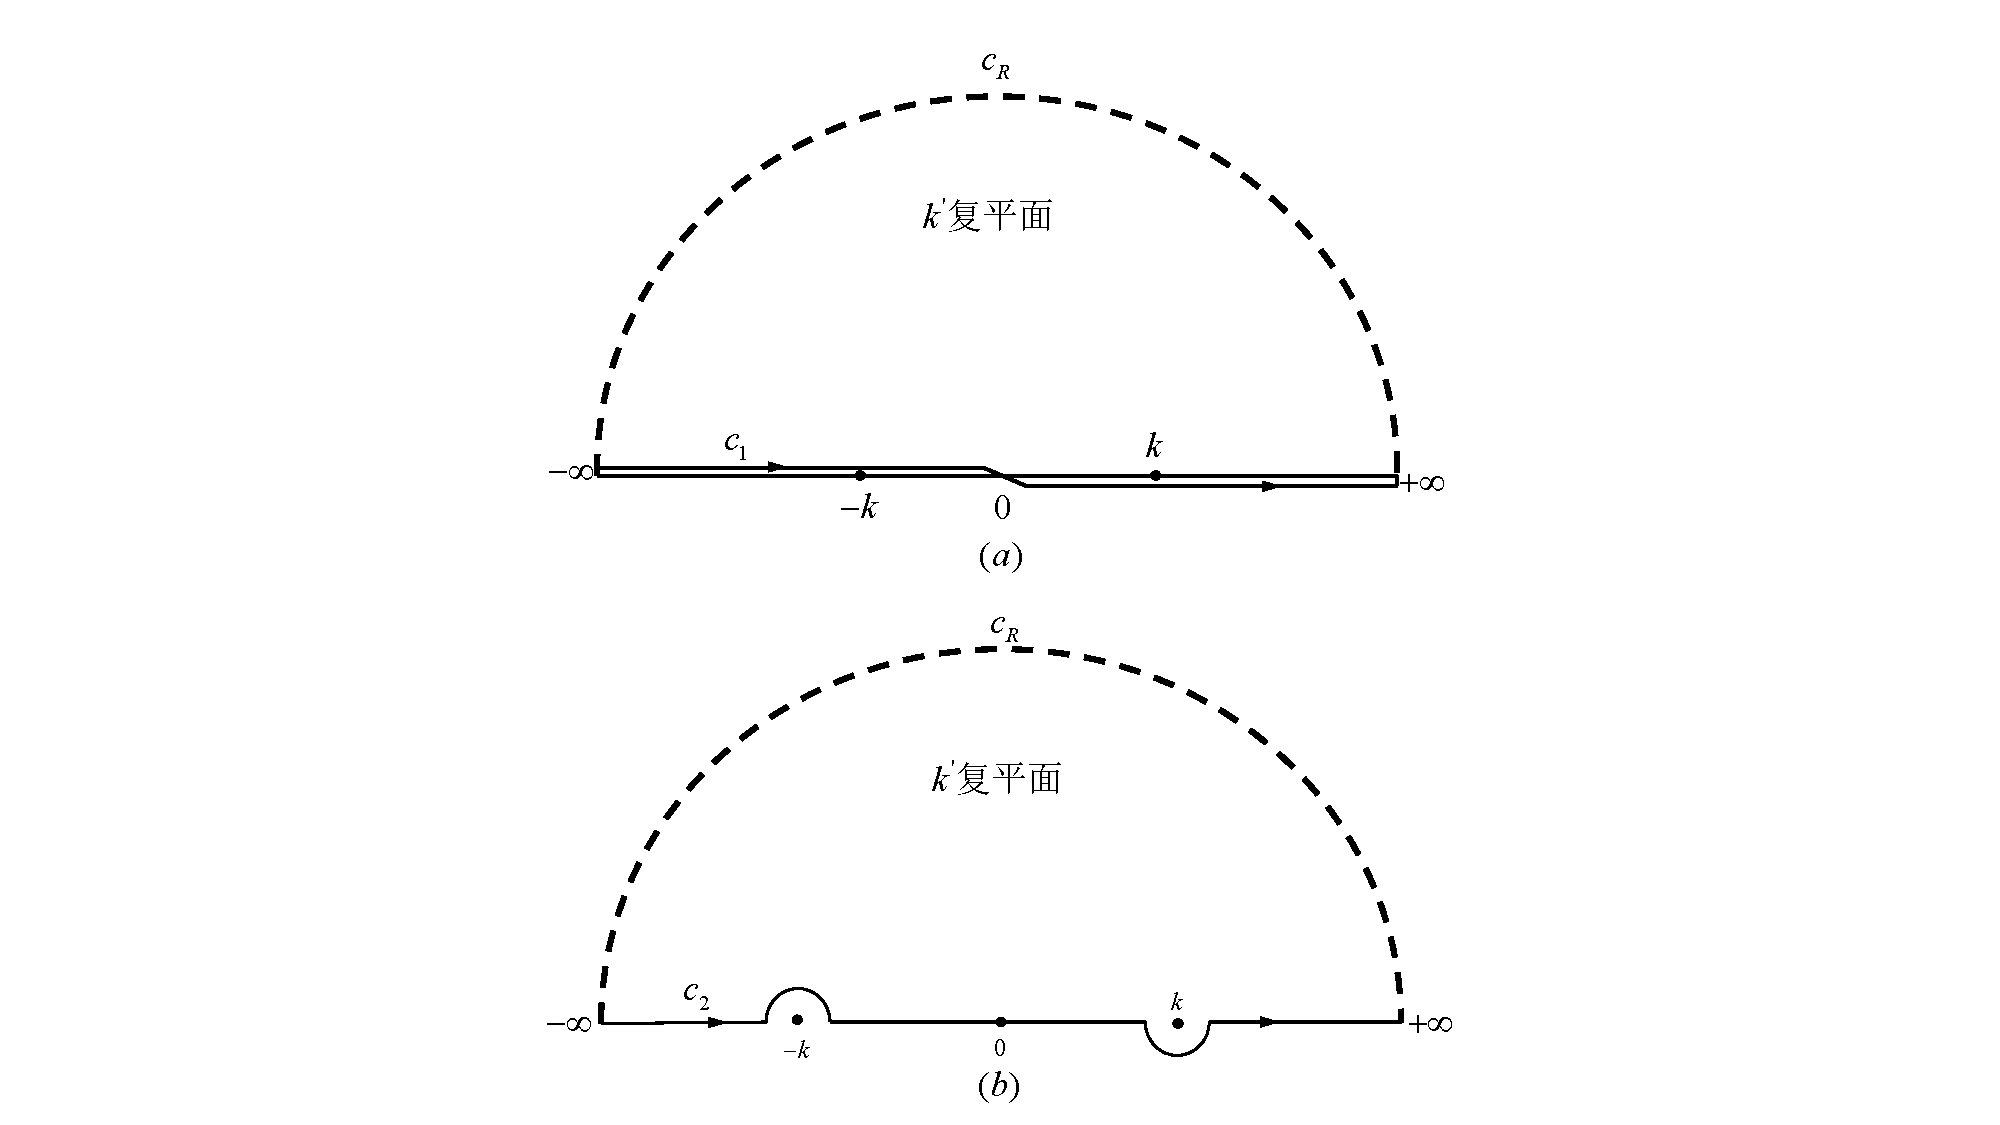
\includegraphics[width=5.5cm,clip]{QM file/figure/8-5}
	\caption{}\label{fig.8-5}
\end{figure}
上式可用$\boldsymbol{k}^{\prime}$复平面上围道积分法算出.但$k^{\prime}=\pm k$是被积函数的一级极点,为了确保$G(\boldsymbol{r},\boldsymbol{r}^{\prime})$中只有出射波,[这样才能符合边界条件\eqref{eq84.7}式]在$\boldsymbol{k}^{\prime}$复平面的左半,积分路线应取实轴上岸,在$\boldsymbol{k}^{\prime}$复平面的右半,积分路线应取实轴下岸,如图\ref{fig.8-5}(a)所示,亦即\eqref{eq84.20}式中积分路线规定为
\begin{empheq}{equation}\label{eq84.21}
	\int_{-\infty}^{\infty}\cdots dk^{\prime}\Rightarrow\int_{c_{1}}\cdots dk^{\prime}
\end{empheq}
这个规定等价于\eqref{eq84.20}式中$k$换成$k+i\varepsilon$($\varepsilon$为无限小正实数) ,或等价于沿图\ref{fig.8-5}(b)中路径$c_{2}$的积分.注意,图\ref{fig.8-5}中沿大圆弧$c_{R}$的积分为0.按照复平面围道积分的残数定理,容易算出
\begin{empheq}{equation}\label{eq84.22}
	\boxed{G(\boldsymbol{r},\boldsymbol{r}^{\prime})=-\frac{\exp(ik|\boldsymbol{r}-\boldsymbol{r}^{\prime}|)}{4\pi|\boldsymbol{r}-\boldsymbol{r}^{\prime}|}}
\end{empheq}
这正是符合散射波性质的出射波形式格林函数.反之,如取积分路径为图\ref{fig.8-5}中(a)实轴下岸及(b)实轴上岸,[相当于\eqref{eq84.20}式中$k$换成$k+i\varepsilon$]则给出
\begin{empheq}{equation*}
	G(\boldsymbol{r},\boldsymbol{r}^{\prime})=-\frac{\exp(ik|\boldsymbol{r}-\boldsymbol{r}^{\prime}|)}{4\pi|\boldsymbol{r}-\boldsymbol{r}^{\prime}|}
\end{empheq}
就不符合散射波的性质,不能采用.


{\heiti 3. 玻恩近似}

将格林函数\eqref{eq84.22}式代入\eqref{eq84.16}式,得到$\varPsi^{(1)}$的明显表示式
\eqlong
\begin{empheq}{equation}\label{eq84.23}
	\varPsi^{(1)}=-\frac{\mu}{2\pi\hbar^{2}}\int\frac{\exp(ik|\boldsymbol{r}-\boldsymbol{r}^{\prime}|)}{|\boldsymbol{r}-\boldsymbol{r}^{\prime}|}V(\boldsymbol{r}^{\prime})\varPsi^{(0)}(\boldsymbol{r}^{\prime})d^{3}\boldsymbol{r}^{\prime}
\end{empheq}\eqnormal
为了得到散射振幅的一级近似$f^{(1)}$,只需要求出$r\rightarrow\infty$处$\varPsi^{(1)}$的函数形式,由于$r\gg r^{\prime}$,可以取下列近似(参看图\ref{fig.8-6}):
\begin{empheq}{equation}\label{eq84.24}
	k|\boldsymbol{r}-\boldsymbol{r}^{\prime}|\approx k\bigg(r-\frac{\boldsymbol{r}^{\prime}\cdot\boldsymbol{r}}{r}\bigg)=kr-\boldsymbol{k}\cdot\boldsymbol{r}^{\prime}
\end{empheq}

\begin{figure}[!h]
	\centering
	\small
	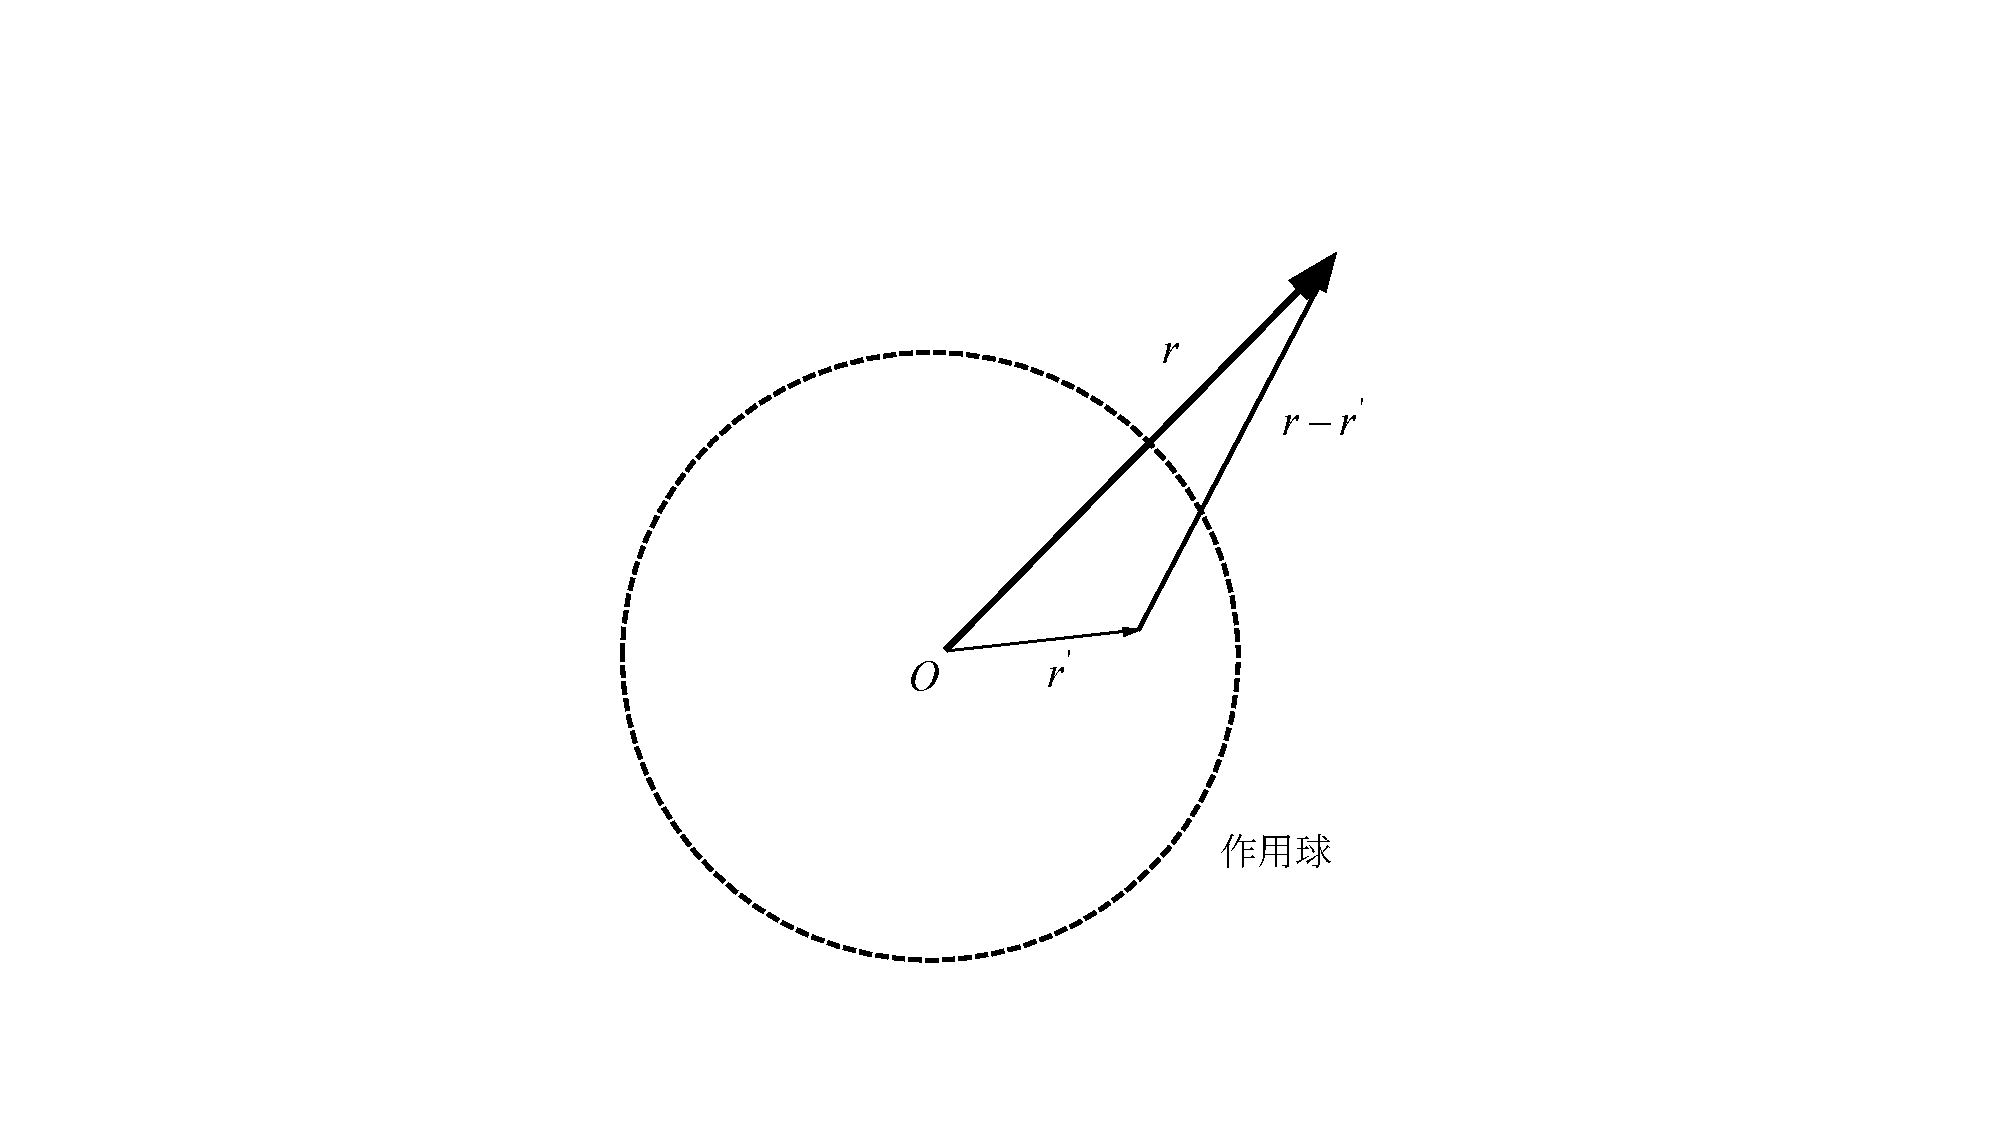
\includegraphics[width=5cm,clip]{QM file/figure/8-6}
	\caption{}\label{fig.8-6}
\end{figure}
$\boldsymbol{k}$为出射波波矢量,其方向即$\boldsymbol{r}$的方向,$\boldsymbol{k}=k\frac{\boldsymbol{r}}{r}$.对于\eqref{eq84.5}式及\eqref{eq84.23}式中的入射波波函数,可表示成
\begin{empheq}{align*}
	\varPsi^{(0)(\boldsymbol{r})}&=e^{ikz}=e^{i\boldsymbol{k}_{0}\cdot\boldsymbol{r}}	\tag{$8.4.5^{\prime}$}\label{eq84.5'}\\
	\varPsi^{(0)(\boldsymbol{r}^{\prime})}&=e^{ikz^{\prime}}=e^{i\boldsymbol{k}_{0}\cdot\boldsymbol{r}^{\prime}}	\tag{$8.4.5^{\prime\prime}$}\label{eq84.5''}\\
\end{empheq}
\noindent$k_{0}$为入射波波矢量,其方向即$z$轴及$z^{\prime}$轴方向.将\eqref{eq84.24}式及\eqref{eq84.5''}式代入\eqref{eq84.23}式,并取\eqref{eq84.23}式中分母$|\boldsymbol{r}-\boldsymbol{r}^{\prime}|$$\approx r$,得到
\eqlong
\begin{empheq}{align}\label{eq84.25}
	\varPsi^{(1)}(\boldsymbol{r}) &\approx-\frac{\mu}{2\pi\hbar^{2}}\frac{e^{ikr}}{r}\int V(\boldsymbol{r}^{\prime})\exp[i(\boldsymbol{k_{0}}-\boldsymbol{k})\cdot\boldsymbol{r}^{\prime}]d^{3}\boldsymbol{r}^{\prime}	\nonumber\\
	&=-\frac{\mu}{2\pi\hbar^{2}}V(\boldsymbol{k},\boldsymbol{k_{0}})\frac{e^{ikr}}{r}
\end{empheq}
\eqnormal
其中
\begin{empheq}{equation}\label{eq84.26}
	V(\boldsymbol{k},\boldsymbol{k_{0}})=\int V(\boldsymbol{r}^{\prime})\exp[i(\boldsymbol{k_{0}}-\boldsymbol{k})\cdot\boldsymbol{r}^{\prime}]d^{3}\boldsymbol{r}^{\prime}
\end{empheq}
比较\eqref{eq84.7}式及\eqref{eq84.25}式,即得散射振幅的一级近似:
\begin{empheq}{equation}\label{eq84.27}
	\boxed{f^{(1)}(\theta,\varphi)=-\frac{\mu}{2\pi\hbar^{2}}V(\boldsymbol{k},\boldsymbol{k_{0}})	}
\end{empheq}
$\boldsymbol{k}$的方向即$(\theta,\varphi)$方向.$(\hbar\boldsymbol{k}-\hbar\boldsymbol{k_{0}})$是散射过程中粒子的动量变化,常被称为“动量转移”,记为$\hbar q$,即
\begin{empheq}{equation}\label{eq84.28}
	\boxed{\boldsymbol{q}=\boldsymbol{k}-\boldsymbol{k_{0}},\quad q=2k\sin\frac{\theta}{2}	}
\end{empheq}

\begin{wrapfigure}[9]{r}{8em}
	\centering
	\small
	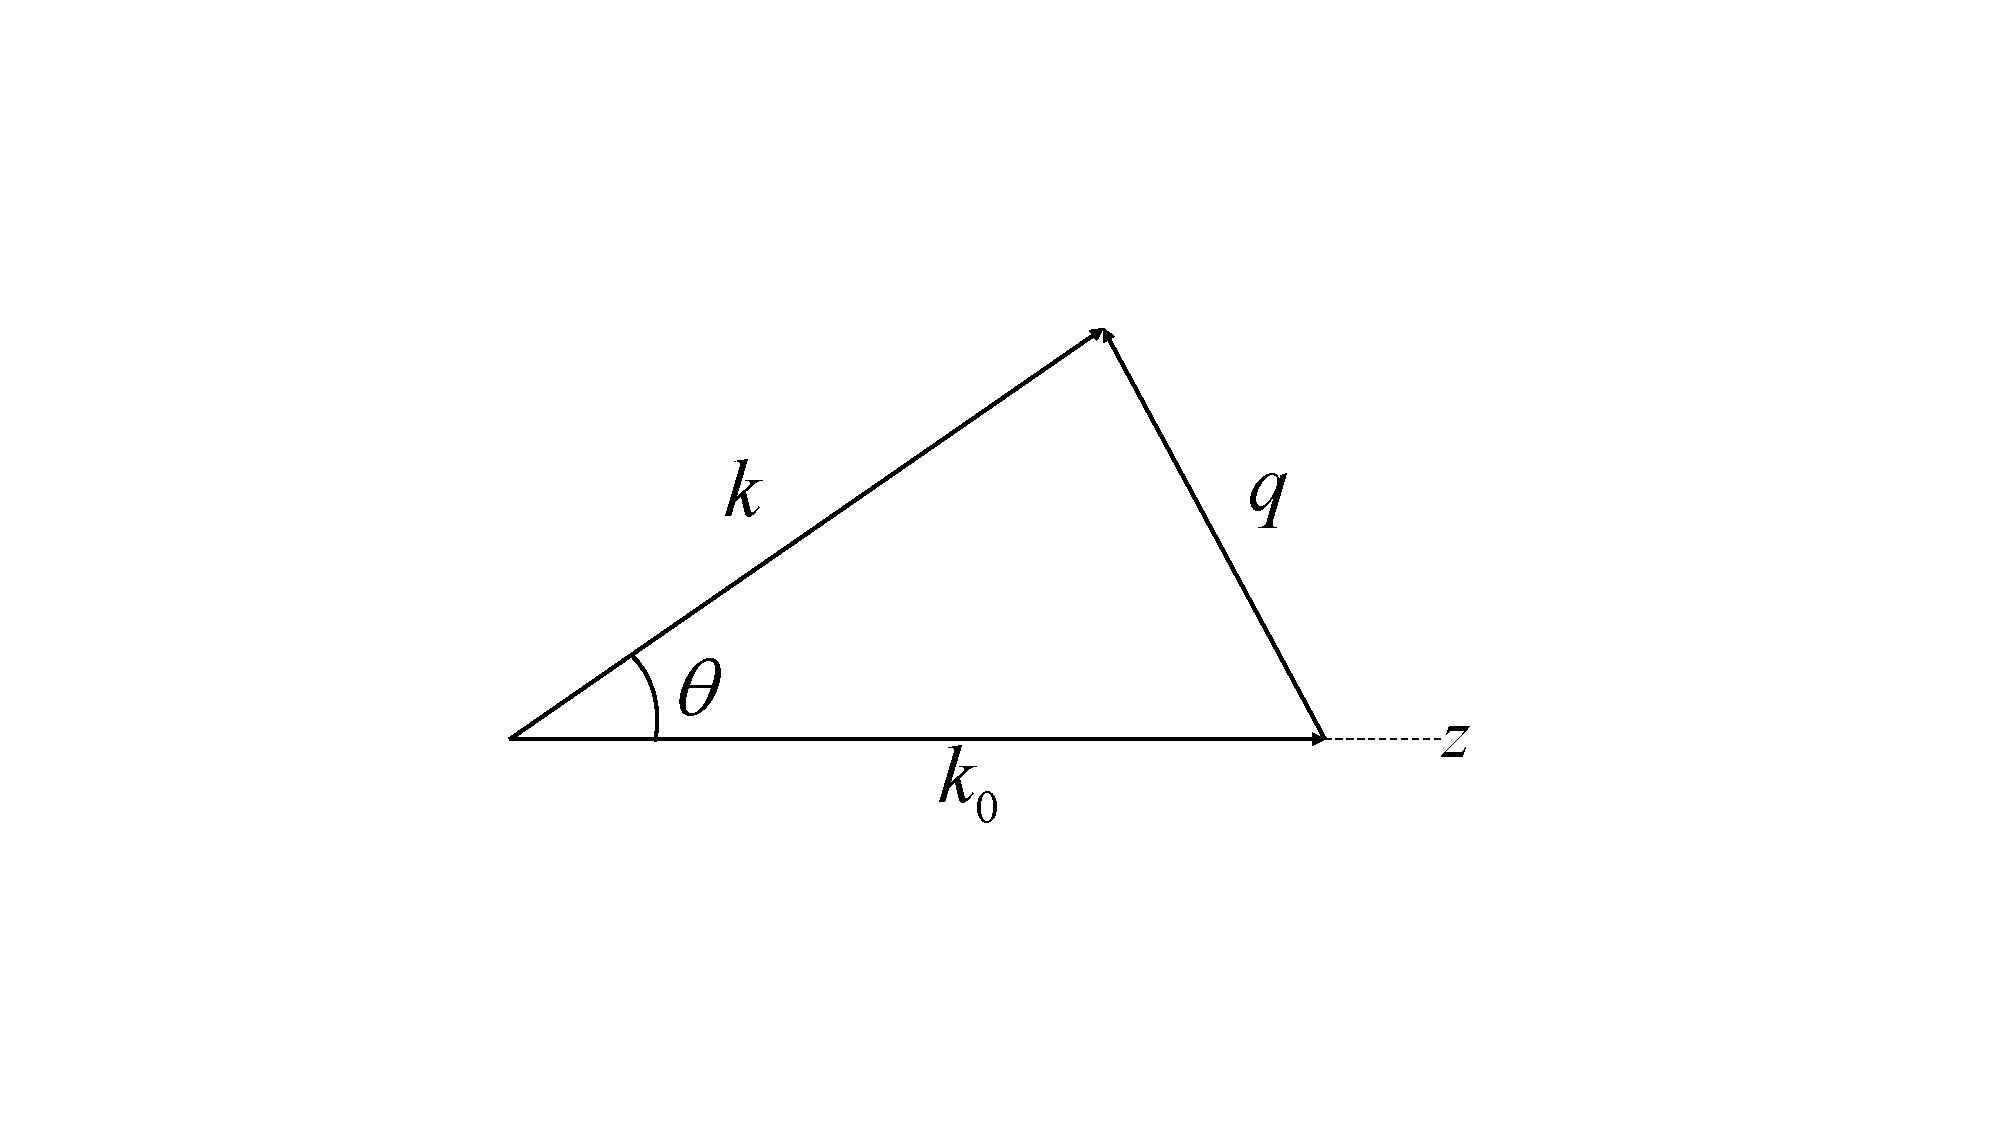
\includegraphics[width=3cm,clip]{QM file/figure/8-7}
	\caption{}\label{fig.8-7}
\end{wrapfigure}
如图\ref{fig.8-7}所示,用$\boldsymbol{q}$代替$(\boldsymbol{k}-\boldsymbol{k_{0}})$,\eqref{eq84.26}式可以写成
\eqindent{4}
\begin{empheq}{equation*}\label{eq84.26'}
	V(\boldsymbol{k},\boldsymbol{k_{0}})=\int V(\boldsymbol{r}^{\prime})	e^{-i\boldsymbol{q}\cdot\boldsymbol{r}^{\prime}}	d^{3}\boldsymbol{r}^{\prime}	\tag{$8.4.26^{\prime}$}
\end{empheq}\eqnormal

如果是中心力散射,$V(\boldsymbol{r}^{\prime})=V(r^{\prime})$,\eqref{eq84.26'}式中角部积分与$V$无关,可以直接算出,如下.$\boldsymbol{r}^{\prime}$空间用球坐标,并以$-\boldsymbol{q}$方向作为极轴方向,则$$-\boldsymbol{q}\cdot\boldsymbol{r}^{\prime}=qr^{\prime}\cos\theta^{\prime},\quad d^{3}\boldsymbol{r}^{\prime}=r^{\prime2}dr^{\prime}\sin\theta^{\prime}d\theta^{\prime}d\varphi^{\prime}$$
\eqlong
\begin{empheq}{align}\label{eq84.29}
	\int e^{-i\boldsymbol{q}\cdot\boldsymbol{r}^{\prime}}\sin\theta^{\prime}d\theta^{\prime}d\varphi&=2\pi\int_{0}^{\pi}e^{iqr^{\prime}\cos\theta^{\prime}}\sin\theta^{\prime}d\theta^{\prime}	\nonumber\\
	&=\frac{4\pi}{qr^{\prime}}\sin qr^{\prime}
\end{empheq}\eqnormal
因此
\begin{empheq}{equation}\label{eq84.30}
	V(\boldsymbol{k},\boldsymbol{k_{0}})=4\pi\int_{0}^{\infty}V(r^{\prime})\frac{\sin qr^{\prime}}{qr^{\prime}}r^{\prime2}dr^{\prime}
\end{empheq}
\begin{empheq}{equation}\label{eq84.31}
	\boxed{f^{(1)}(\theta)=-\frac{2\mu}{\hbar^{2}}\int_{0}^{\infty}V(r^{\prime})\frac{\sin qr^{\prime}}{qr^{\prime}}r^{\prime2}dr^{\prime}	}
\end{empheq}
由于$q=2k\sin\bigg(\frac{\theta}{2}\bigg)$,所以$f^{(1)}$是散射角$\theta$的函数.

如果略去二级修正,则微分散射截面为
\begin{empheq}{equation}\label{eq84.32}
	\sigma(\theta,\varphi)\approx|f^{(1)}|^{2}=\frac{\mu^{4}}{4\pi^{2}\hbar^{4}}|V(\boldsymbol{k},\boldsymbol{k_{0}})|^{2}
\end{empheq}
对于中心力场散射,微分散射截面仅为$\theta$的函数,
\begin{empheq}{equation}\label{eq84.33}
	\sigma(\theta)\approx\frac{4\mu^{2}}{\hbar^{4}}\bigg[\int_{0}^{\infty}V(r^{\prime})\frac{\sin qr^{\prime}}{qr^{\prime}}r^{\prime2}dr^{\prime}\bigg]^{2}
\end{empheq}
以上结果[主要指\eqref{eq84.25}、\eqref{eq84.27}、\eqref{eq84.32}式]通常称为玻恩(M.Born)近似.

{\heiti 4. 玻恩近似的适用条件}

\eqref{eq84.2}式或\eqref{eq84.10}式的严格解应该写成
\begin{empheq}{align*}\label{eq84.10'}
	\varPsi_{s}(\boldsymbol{r}) &=(\nabla^{2}+k^{2})^{-1}\frac{2\mu}{\hbar^{2}}V(\boldsymbol{r})\varPsi(\boldsymbol{r})	\\
	&=\frac{2\mu}{\hbar^{2}}\int G(\boldsymbol{r},\boldsymbol{r}^{\prime})V(\boldsymbol{r}^{\prime})\varPsi(\boldsymbol{r}^{\prime})d^{3}\boldsymbol{r}^{\prime}
	\tag{$8.4.10^{\prime}$}
\end{empheq}
由于$\varPsi=\varPsi^{(0)}+\varPsi_{s}$,上式为积分方程\eqref{eq84.16}式是上式的一级近似解,相当于在右端的积分中以$\varPsi^{(0)}$代替$\varPsi$.由此可知\eqref{eq84.16}式和\eqref{eq84.23}式的适用条件是在散射区内$(r\sim r^{\prime})|\varPsi^{(1)}(\boldsymbol{r})|\ll|\varPsi^{(0)}(\boldsymbol{r})|$,亦即
\begin{empheq}{equation}\label{eq84.34}
	|\varPsi^{(1)}(\boldsymbol{r})|\ll1\quad (r\sim r^{\prime})
\end{empheq}
通常,作用势$V(\boldsymbol{r}^{\prime})$总是存在一定的有效范围(作用球,半径$a$),在作用球内,$V$变化平缓,在作用球外,$V$迅速减弱.作为数量级估算,\eqref{eq84.23}式中$V(\boldsymbol{r}^{\prime})$不妨用平均值$V_{0}$来代替,而积分在作用球内进行.这样做相当于采用球形势垒(阱)模型.通常,在力心附近$(r\sim 0)$散射作用较强,所以\eqref{eq84.34}式可取$r=0$进行估算,即适用条件取为
\eqlong
\begin{empheq}{equation}\label{eq84.35}
	|\varPsi^{(1)}(0)|\approx\frac{\mu|V_{0}|}{2\pi\hbar^{2}}\bigg|\int\frac{d^{3}\boldsymbol{r}^{\prime}}{r^{\prime}}\exp[ikr^{\prime}+i\boldsymbol{k_{0}}\cdot\boldsymbol{r}^{\prime}]\bigg|\ll1
\end{empheq}\eqnormal
其中$\exp(i\boldsymbol{k_{0}}\cdot\boldsymbol{r}^{\prime})=\exp(ikz^{\prime})=\varPsi^{(0)}(\boldsymbol{r}^{\prime})$.

对于低能散射,$ka\ll 1$,\eqref{eq84.35}式中指数函数近似等于1,而
\begin{empheq}{equation*}
	\int\frac{d^{3}\boldsymbol{r}^{\prime}}{r^{\prime}}\approx4\pi\int_{0}^{a}r^{\prime}d^{\prime}=2\pi a^{2}
\end{empheq}
所以适用条件为
\begin{empheq}{equation}\label{eq84.36}
	|\varPsi^{(1)}(0)|\approx \mu|V_{0}|\frac{a^{2}}{\hbar^{2}}\ll1
\end{empheq}
要满足此式,势垒(阱)必须充分弱($|V_{0}|$小)而窄($a$小).

对于高能散射,$ka\gg1$,\eqref{eq84.35}式中指数函数在$0<r^{\prime}<a$范围内将多次振荡,必须作出较精确的估算,采用球坐标$(r^{\prime},\theta^{\prime},\varphi^{\prime})$,将\eqref{eq84.35}式中角部积分算出[参看\eqref{eq84.29}式],
\begin{empheq}{equation*}
	\int e^{i\boldsymbol{k}_{0}\cdot\boldsymbol{r}}\sin\theta^{\prime}d\varphi^{\prime}=4\pi\frac{\sin kr^{\prime}}{kr^{\prime}}
\end{empheq}
所以
\eqlong
\begin{empheq}{align}\label{eq84.37}
	&\int\frac{d^{3}\boldsymbol{r}^{\prime}}{r^{\prime}}\exp(ikr^{\prime}+i\boldsymbol{k_{0}}\cdot\boldsymbol{r}^{\prime})=\frac{4\pi}{k}\int_{0}^{a}\sin kr^{\prime}e^{ikr^{\prime}}dr^{\prime}	\nonumber\\
	=&\frac{4\pi}{k^{2}}\int_{0}^{ak}\sin xe^{ix}dx=\frac{4\pi}{k^{2}}\bigg[\frac{i}{2}ak+\frac{1}{4}(1-e^{2iak})\bigg]	\nonumber\\
	=&\frac{4\pi}{k^{2}}\cdot\frac{i}{2}ak=2i\pi\frac{a}{k}
\end{empheq}\eqnormal
代入\eqref{eq84.35},即得适用条件为
\begin{empheq}{equation}\label{eq84.38}
	|\varPsi^{(1)}(0)|\approx \mu|V_{0}|\frac{a}{\hbar^{2}k}\ll1
\end{empheq}
即
\begin{empheq}{equation*}\label{eq84.38'}
	\mu|V_{0}|\frac{a^{2}}{\hbar^{2}}\ll ak\quad\text{或}\quad 2|V_{0}|ak\ll\frac{\hbar^{2}k^{2}}{2\mu}=E
	\tag{$8.4.38^{\prime}$}
\end{empheq}
显然,入射粒子的动能$\bigg(E=\frac{\hbar^{2}k^{2}}{2\mu}\bigg)$越大,条件\eqref{eq84.38'}越易满足.注意,对于一定的势场$(V_{0},a)$,玻恩近似是否适用于低能散射,即\eqref{eq84.36}式是否成立,是由势场本身决定的;而对于高能散射,只要入射能量足够大,总能使\eqref{eq84.38}式成立,即玻恩近似可以适用.另外,比较\eqref{eq84.36}及\eqref{eq84.38}式,可知$|\varPsi^{(1)}(0)|^{2}$之值在高能散射时约为低能散射时的$(ak)^{-2}$倍,由此可以估计,两种情况下总散射截面大致也相差$(ak)^{-2}$倍.

顺便讨论一下中心力散射的玻恩近似\eqref{eq84.31}、\eqref{eq84.33}式.在低能散射条件$(ka\ll1)$下,对于任何散射$\theta$,均有
\begin{empheq}{align*}
	qr^{\prime}=2kr^{\prime}&\sin\bigg(\frac{\theta}{2}\bigg)<2ka\ll1	\\
	&\frac{\sin qr^{\prime}}{qr^{\prime}}\approx 1
\end{empheq}
\eqref{eq84.31}式给出
\begin{empheq}{equation}\label{eq84.39}
	f^{(1)}\approx -\frac{2\mu}{\hbar^{2}}\int_{0}^{\infty}V(r^{\prime})r^{\prime2}dr^{\prime}
\end{empheq}
$f(\theta)\approx f^{(1)}$与$\theta$无关,这结果相当于分波法中低能s波$(l=0)$散射.例如对于球形势阱$(V=-V_{0},r<a)$,上式给出
\begin{empheq}{align}\label{eq84.40}
	&f(\theta)\approx f^{(1)}\approx\frac{2\mu V_{0}a^{3}}{3\hbar^{2}}		\nonumber\\
	\sigma_{\text{总}}&\approx 4\pi|f|^{2}=\frac{16\pi}{9}\bigg(\frac{\mu V_{0}a^{3}}{\hbar^{2}}\bigg)^{2}
\end{empheq}
这正是\eqref{eq83.21}式.$\S$\ref{sec:08.03}例题中提到的条件$ka\ll1$,正是玻恩近似的适用条件,即本节\eqref{eq84.36}式注意,由于条件\eqref{eq84.36}式,$\sigma_{\text{总}}\ll\pi a^{2}$.

仍以球形势阱(或势垒,强度$V_{0}$,半径$a$)为例,对高能散射作定性讨论.\eqref{eq84.31}式中以$\pm V_{0}$代替$V(r^{\prime})$后,积分可以简单算出,
\eqlong
\begin{empheq}{align}\label{eq84.41}
	&\int_{0}^{a}\frac{\sin qr^{\prime}}{qr^{\prime}}r^{\prime2}dr^{\prime}=q^{-3}\int_{0}^{aq}x\sin xdx		\nonumber\\
	=&a^{3}(\sin aq-aq\cos a)(aq)^{-3}=a^{3}F(aq)
\end{empheq}\eqnormal
其中$a_{q}=2ak\sin\bigg(\frac{\theta}{2}\bigg)$.当$aq<\pi$,$F(aq)$随$aq$之增大而徐缓减小,$(aq=0.1,F=0.33;aq=1,F=0.30;aq=2,F=0.22;aq=\pi,F=0,10)$当$aq>\pi$,$|F(aq)|$迅速减小$(aq=4.49,F\sim0;aq=5,F=-\num{0.019};aq=2\pi,F=-\num{0.025};aq=3\pi,F=\num{0.011})$.因此,仅当$\theta<\pi/ak(aq\sim ak\theta<\pi)$,$f(\theta)$及$\sigma(\theta)$才有显著的值(但对$\theta$的变化不敏感).这就是说,在玻恩近似成立的前提下,大部分散射粒子的散射角$\theta<\frac{\pi}{ak}$.相应的$f(\theta)$约为
\begin{empheq}{align}\label{eq84.42}
	|f(\theta)|\approx \frac{2\mu V_{0}a^{3}}{\hbar^{2}}F(aq)\lesssim\frac{2\mu V_{0}a^{3}}{3\hbar^{2}}
\end{empheq}
$\bigg(F\lesssim\frac{1}{3}\bigg)$而总散射截面约为
\begin{empheq}{align}\label{eq84.43}
	\sigma_{\text{总}} &=\int|f(\theta)|^{2}\sin\theta d\theta d\varphi	\nonumber\\
	&\lesssim\bigg(\frac{2\mu V_{0}a^{3}}{3\hbar^{2}}\bigg)^{2}2\pi\int_{0}^{\frac{\pi}{ak}}\sin\theta d\theta	\nonumber\\
	&\sim \bigg(\frac{2\mu V_{0}a^{3}}{3\hbar^{2}}\bigg)\frac{\pi^{3}}{(ak)^{2}}\propto\frac{1}{k^{2}}\propto\frac{1}{E}
\end{empheq}
按量级说,大致是低能$\sigma_{\text{总}}$的$(ak)^{-2}$倍.注意,由于条件\eqref{eq84.38'}式,易见$\sigma_{\text{总}}\ll4\pi a^{2}$,这意味着散射是微弱的.而且,$\sigma_{\text{总}}$大体上与$E$成反比.
\pskip

\example 质量为$\mu$的粒子束以动量$\hbar k$入射,遇中心力场
\begin{empheq}{equation}\label{eq84.44}
	V(r)=\frac{B}{r}e^{-r/a}\quad (a>0)
\end{empheq}
求散射截面的玻恩近似(一级近似).并讨论$ka\gg1,ka\ll1,a\rightarrow\infty$等极限情形.

\solution 在玻恩近似下,散射振幅由\eqref{eq84.31}式表示,即
\begin{empheq}{align}\label{eq84.45}
	f(\theta) &=-\frac{2\mu B}{\hbar^{2}q}\int_{0}^{\infty}\sin qre^{-r/a}dr	\nonumber\\
	&=-\frac{2\mu B}{\hbar^{2}q}\cdot\frac{qa^{2}}{1+q^{2}a^{2}}	\nonumber\\
	&=-\frac{2\mu Ba^{2}}{\hbar^{2}}\cdot\frac{1}
	{1+4a^{2}k^{2}\sin^{2}\bigg(\frac{\theta}{2}\bigg)}
\end{empheq}
微分散射截面及总散射截面为
\begin{empheq}{equation*}
	\sigma(\theta)=|f(\theta)|^{2},\quad \sigma_{\text{总}}=2\pi\int_{0}^{\pi}\sigma(\theta)\sin\theta d\theta
\end{empheq}
可以算出
\begin{empheq}{equation}\label{eq84.46}
	\sigma_{\text{总}}=\frac{16\pi\mu^{2}B^{2}a^{4}}{\hbar^{2}(1+4a^{2}k^{2})}
\end{empheq}
由\eqref{eq84.44}式表示的作用势,可以用于许多问题.反映核子-核子作用力的“汤川(Yukawa)势”正是这种形式,$a$代表力程$(a\sim 2\si{fm})$,$B/a$代表平均作用强度(约$20\sim30\si{MeV}$).带电粒子被原子散射,\eqref{eq84.44}式可以近似表示“屏蔽库仑势”,因子$e^{-r/a}$代表原子的电子壳层对于核电荷的屏蔽效应($a\sim$原子半径).纯库仑势$V\propto\frac{1}{r}$,相当于$a\rightarrow\infty$这种极端的情形.

高能散射,$ka\gg1$,在\eqref{eq84.45}式中只要$\theta$不太小,能使$qa\gg1$,则
\begin{empheq}{align}
	f(\theta) &\approx-\frac{\mu B}{2\hbar^{2}k^{2}\sin^{2}\bigg(\frac{\theta}{2}\bigg)}				\label{eq84.47}\\
	\sigma(\theta)
	&\approx\frac{\mu^{2}B^{2}}{4\hbar^{4}k^{4}\sin^{4}\bigg(\frac{\theta}{2}\bigg)}\nonumber\\
	&=\frac{B^{2}}{16E^{2}\sin^{4}\bigg(\frac{\theta}{2}\bigg)} \label{eq84.48}
\end{empheq}
这结果相当于$a\rightarrow\infty$的情况,即纯库仑势散射.但是,对于纯库仑势,上式也适用于很小的散射角,因此$\sigma_{\text{总}}\rightarrow\infty$.而对于力程$\theta$有限的情况,\eqref{eq84.48}式只适用于$qa\gg1$,即$\theta\gg\frac{1}{ka}$.当$\theta\rightarrow0$,\eqref{eq84.45}式给出$f(0)=-\frac{2\mu Ba^{2}}{\hbar^{2}}$,为有限值.\eqref{eq84.46}式在$ka\gg1$条件下给出
\begin{empheq}{equation}\label{eq84.49}
	\sigma_{\text{总}}\overset{ka\gg1}{\longrightarrow}4\pi\frac{\mu^{2}B^{2}a^{2}}{\hbar^{4}k^{2}}\propto\frac{1}{E}
\end{empheq}
这结果与\eqref{eq84.43}式大致符合$(B\sim V_{0}a)$.

低能散射,$ka\ll1$,对任何散射角$\theta$,均有$qa\gg1$,\eqref{eq84.45}式给出
\begin{empheq}{equation}\label{eq84.50}
	f(\theta)\approx -\frac{2\mu Ba^{2}}{\hbar^{2}},\quad \sigma(\theta)\approx \frac{4\mu^{2}B^{2}a^{4}}{\hbar^{4}}
\end{empheq}
$\sigma(\theta)$与$\theta$无关,这是低能散射的特点.在$ka\ll1$条件下,玻恩近似的适用条件为
\eqlong
\begin{empheq}{equation}\label{eq84.51}
	|\varPsi_{s}(0)|\approx\frac{2\mu}{\hbar^{2}}\cdot\frac{1}{4\pi}\bigg|\int V(\boldsymbol{r})\frac{d^{3}\boldsymbol{r}}{r}\bigg|=\frac{2\mu a}{\hbar^{2}}|B|\ll1
\end{empheq}\eqnormal
所以
\begin{empheq}{equation*}
	\sigma_{\text{总}}=4\pi\sigma(\theta)=4\pi a^{2}\bigg(\frac{2\mu Ba}{\hbar^{2}}\bigg)^{2}\ll 4\pi a^{2}
\end{empheq}

在许多问题中,条件\eqref{eq84.51}往往不成立.例如核子-核子散射,$a\sim2\si{fm},\frac{B}{a}\sim30\si{MeV},2\mu c^{2}\sim938\si{MeV}$,则
\eqlong
\begin{empheq}{equation*}
	\frac{2\mu Ba}{\hbar^{2}}=\frac{2\mu c^{2}Ba}{(\hbar c)^{2}}\sim\frac{938\times30\times4(\si{MeV}\cdot\si{fm})^{2}}{(200\si{MeV}\cdot\si{fm})^{2}}\sim 2.8
\end{empheq}\eqnormal
所以核子-核子低能散射一般不能用玻恩近似处理,而必须用分波法.




% 习题
\begin{exercises}
	
\exercise 粒子束被中心势场$V(r)=\dfrac{\alpha}{r^{2}}(\alpha>0)$散射,求各分波相移$\delta_{l}$.再在条件$\dfrac{\mu\alpha}{\hbar^{2}}\ll\dfrac{1}{8}$下,求$\delta_{l},f(\theta)$及$\sigma(\theta)$的近似公式.

[提示:将$V(r)$与离心势能合成一项,$l$分波径向函数可以表示成$R_{l}(r)=\sqrt{\dfrac{\pi}{2kr}}J_{\nu+\frac{1}{2}}(kr)$的形式,找出$\nu$与$l$的关系.

近似处理时利用公式$\dfrac{1}{\sin\bigg(\dfrac{\theta}{2}\bigg)}=2\sum_{l=0}^{\infty}P_{l}(\cos\theta)$.]
	
\exercise 势场同上题,用玻恩近似公式计算散射振幅及微分散射截面.
	
\exercise 粒子束被球形势阱散射,
\begin{equation*}
	V(r)=\begin{cases}
		-V_{0}, \quad&r<a	\\
		0,\quad &r>a
	\end{cases}
\end{equation*}
设$\dfrac{2\mu V_{0}a^{2}}{\hbar^{2}}\ll1$,并考虑低能散射$(ka\ll1)$.

(a) 用\eqref{eq82.26}式计算s波$(l=0)$相移$\delta_{0}$及散射振幅,总散射截面.

(b) 用玻恩近似公式计算散射振幅和总散射截面.玻恩近似公式适用的条件是什么?

\exercise 在分波法计算中,如只需考虑$l=0,1$两个分波的散射,试写出$f(\theta)$及$\sigma(\theta)$的公式,并就$\delta_{0}=\dfrac{\pi}{9},\delta_{1}=\dfrac{\pi}{36}$,具体计算$\theta=0,\dfrac{\pi}{2},\pi$三种方向$\sigma(\theta)$的相对比率.
	
\exercise 对于下列中心势场,用玻恩近似计算出$f(\theta)$,$\sigma(\theta)$.

(a)	$V(r)=A\delta(\boldsymbol{r})$ (b) $V(r)=V_{0}e^{-\alpha r}$ (c) $V(r)=V_{0}e^{-\alpha^{2}r^{2}}$
	
\exercise 高速粒子被球壳$\delta$势场$V(r)=B\delta(r-a)$散射,用玻恩近似求$f(\theta)$,$\sigma(\theta)$.
	
\exercise 低速粒子束被势场$V(r)=\dfrac{\alpha}{r^{4}}(\alpha>0)$散射,求$E\rightarrow0$时s波$(l=0)$的散射长度,相移,散射振幅,散射截面.

[提示:本题为长程力,相当于作用球半径为$\infty$,故需在$r\rightarrow\infty$处将$u_{0}(r)$表示成$c\bigg(1-\dfrac{r}{a_{0}}\bigg)$的形式.在这样做之前,先证明$E\rightarrow0$时s波径向方程之解为$u_{0}=xe^{-1/x},x=\dfrac{r\hbar}{\sqrt{2\mu\alpha}}$.]
	
\exercise 粒子被势场$V(r)=-\dfrac{\hbar^{2}}{\mu}\left[\dfrac{\lambda}{\si{ch}(\lambda r)}\right]^{2}$($\lambda>0$,ch$(x)$为双曲余弦函数)散射,求低能$(E\rightarrow0)$s波散射截面.

[提示:证明$u_{0}(r)=\dfrac{\si{sh}(\lambda r)}{\si{ch}(\lambda r)}$.本题为共振散射.]
	
\exercise 某原子的电荷分布各向同性,电荷密度$\rho(r)$在$r\rightarrow+\infty$处迅速趋于0,而且$\int\rho(r)d^{3}\boldsymbol{r}$(总电量为0),$\int\rho(r)r^{2}d^{3}\boldsymbol{r}$(代表分布不均匀性)设有动量$\boldsymbol{p}=\hbar k$的电子束受到这电荷分布所生静电场作用而发生散射.试用玻恩近似公式计算$\theta\sim0$方向的微分散射截面$\sigma(0)$.如原子为基态氢原子,结果如何?

[提示:$\int\cdots d^{3}\boldsymbol{r}$本为全空间积分,为便于处理,积分可在半径$R$($R$充分大)的球内进行.]
	
\exercise 高速电子被原子散射,原子对入射电子的库仑作用势可以近似表示成
\begin{empheq}{equation*}
	V(\boldsymbol{r})=-\frac{Z\e^{2}}{r}+\e^{2}\int\frac{\rho(r^{\prime})}{|\boldsymbol{r}-\boldsymbol{r}^{\prime}|}d^{3}\boldsymbol{r}^{\prime}
\end{empheq}
其中第二项表示原子中的电子分布对入射电子的库仑作用,$(-\e)\rho(\boldsymbol{r}^{\prime})$为电子分布的电荷密度.

(a) 试用玻恩近似公式求散射振幅和微分截面,证明
\begin{empheq}{equation*}
	f(\theta)=\frac{2\mu \e^{2}}{\hbar^{2}q^{2}}[Z-F(q)],\quad F(q)=\int\rho(\boldsymbol{r}^{\prime})e^{-\boldsymbol{q}\cdot\boldsymbol{r}^{\prime}}d^{3}\boldsymbol{r}^{\prime}
\end{empheq}

(b) 电子被氢原子(基态)散射,利用上述公式求$f(\theta)$,并讨论$\theta\ll\dfrac{1}{ka_{0}}$($a_{0}$为玻尔半径)的情形,求$f(\theta),\sigma(\theta)$.

\end{exercises}
